\documentclass{report}
\usepackage[margin=1.25in]{geometry}
\usepackage{hyperref}
\usepackage{amsmath}
\usepackage{amssymb}
\usepackage{amsthm}
\usepackage{listings}
\usepackage{parskip}
\usepackage{graphicx}
\usepackage[center]{caption}

\newcommand\imageheight{10cm}

\newcommand\sds{\spacefactor\sfcode`.\ \space}

\hyphenation{THROW-THOSE-PIC-TURES-DOWN-THE-LANE}

\newtheorem{thm}{Theorem}
\title{+/ Drawings}
\author{Varik Valefor}
\begin{document}
\maketitle{}
\tableofcontents{}
\chapter{le te pavroipli}
.ni'o ti poi te tcidu cu vasru su'o lo lampru pixra poi se zbasu la .varik.\ .valefor.\ ku'o goi ko'a ge'u .e lo datni be ko'a

.i le nu zo su'o se pilno cu krinu le nu su'o da poi se zbasu la .varik.\ .valefor.\ ku'o zo'u selcaugau da ti poi te tcidu\sds  .i le nu selcaugau lo glefi'a pixra poi se zbasu la .varik.\ ku'o ti poi te tcidu cu mupli

\chapter{le plijaspu}
.ni'o so'i da poi pixra gi'e se zbasu la .varik.\ gi'e se vasru ti poi te tcidu zo'u le velski be da ku xusra le du'u la'o gy.\ CC BY-NC 4.0 .gy cu plijaspu da\sds  .i ku'i ro da poi pixra gi'e se zbasu la .varik.\ gi'e se vasru ti poi te tcidu zo'u la .varik.\ pu rinka le nu la'o gy.\ Unlicense .gy cu plijaspu da\sds  .ija'e ro da poi pixra gi'e se zbasu la .varik.\ gi'e se vasru ti poi te tcidu zo'u la'o gy.\ Unlicense .gy cu plijaspu da

\chapter{la'o gy.\ 20200414042645-03 .gy}
\begin{figure}[ht]
	\centering
	
\includegraphics[height=\imageheight]{20200414042645-03/20200414042645-03.jpg}
	\caption[center]{le cipra pixra noi claxu lo xamgu cmene}
\end{figure}
\section{le pamoi ve skicu be le pixra}
.ni'o ti poi pixra cu pu se zbasu ki'u le nu djica le nu jdice le du'u le nu pilno lo skami smacu le nu pixra cu frili kei kei .e le nu la'o gy.\ GIMP .gy xlali samru'e\sds  .i jimpe fa le du'u la'o gy.\ GIMP .gy xlali samru'e kei .e le du'u tcecumki fa le nu pilno lo skami smacu le nu pixra

.ni'o nelci la'o gy.\ dickcissel .gy

\section{la'oi .watermark.}
.ni'o la .varik.\ jinvi le du'u la'oi .watermark.\ po ti poi pixra cu dukse\ldots\sds .i le nu di'u tceje'u cu cabna le nu la .varik.\ pensi le du'u la .varik.\ pu fairgau lo favytcinymupli be fi ti poi pixra poi claxu la'oi .watermark.

\begin{figure}[ht]
	\centering
	
\includegraphics[height=10cm]{20200414042645-03/20200414042645-03-uw.png}
	\caption[center]{.ni'o lo favytcinymupli be le pixra cu se gubyternoi\ldots i le kerfa bo tengu claxu cu go'i\sds  .i rigni}
\end{figure}

\section{le cfila be la'o gy.\ 20200414042645-03 .gy}
le'i cfila be la'o gy.\ 20200414042645-03 .gy goi ko'a cu se cmima
\begin{itemize}
	\item le ka le cnebo be la'oi .VUNC.\ ku poi se pixra ko'a cu claxu
	\begin{itemize}
		\item su'o lo ctino be le stedu be la'oi .VUNC.\ ku ku .e
		\item su'o lo sirsunla tengu kei .e
	\end{itemize}
	\item le ka le galraipau be le se viska pagbu be le zunle kanla be la'oi .VUNC.\ ku ku ku poi se pixra ko'a cu claxu lo ctino
\end{itemize}

\chapter{la'o gy.\ Proactive Security .gy}
\begin{figure}[ht]
	\centering
	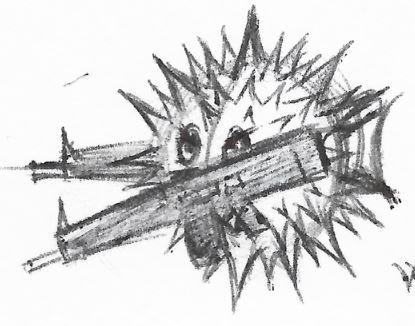
\includegraphics[height=10cm]{proactivesecurity/proactivesecurity.png}
	\caption[center]{.ni'o le nu mi'a pilno la'o gy.\ OpenBSD .gy cu zva'ati\sds  .i doi fazgau do'u ko na troci}
\end{figure}
\section{le pamoi velski be le pixra}
.ni'o la'o gy.\ Proactive Security .gy cu se kibdu'a ki'u le nu filselga'e claxu lo pixra be la .pyfis.

.ni'o la .pyfis.\ claxu lo kalmebykre ki'u le nu mo'ifli le nu pixra lo kalmebykre

.ni'o la'o gy.\ AA-12 .gy .u'enderfu xacyce'a

\chapter{la'o gy.\ WESTERNUNIONSOFTHECOUNTRYWESTERNS .gy}
\begin{figure}[ht]
	\centering
	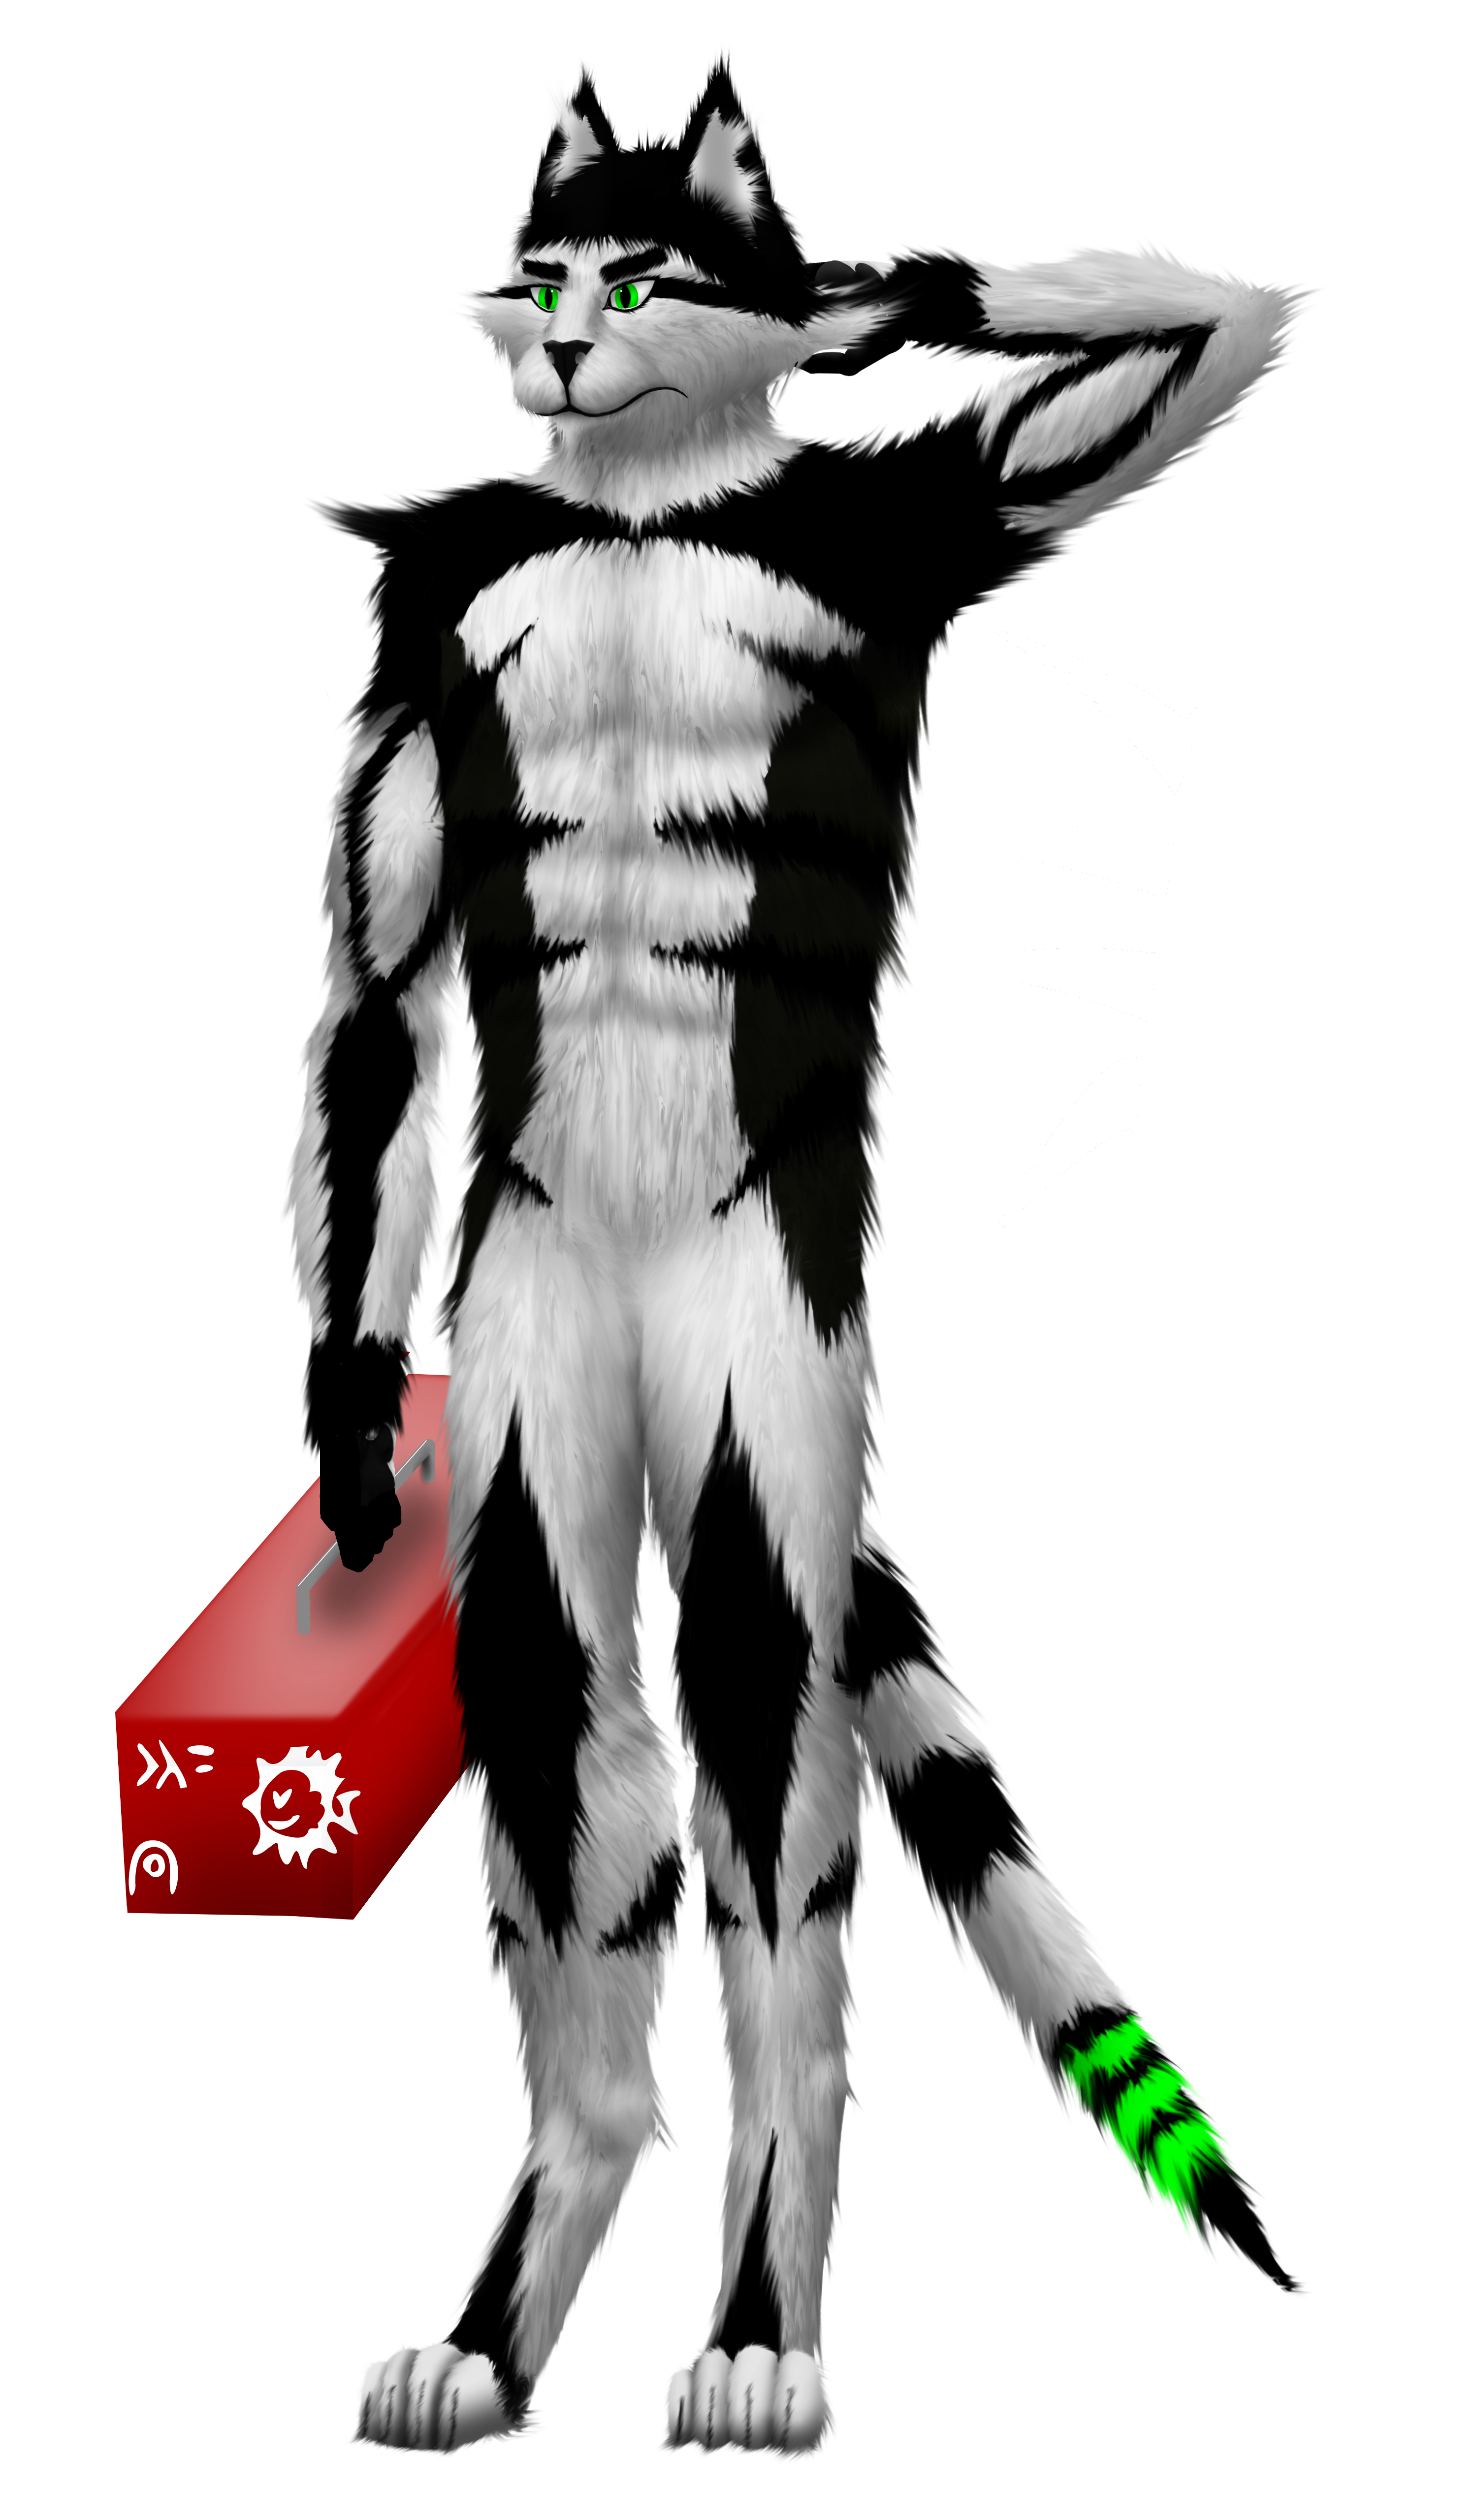
\includegraphics[height=\imageheight]{50x/toolbox/westernunionsofthecountrywesterns.png}
	\caption[center]{le pixra .e le na se tcidu}
\end{figure}
\section{le pamoi velski be le pixra}
\subsection{lo snada ci fi'u vo zo'e}
.ni'o le nu la .varik.\ troci le nu terxra lo ci fi'u vo xarpre be la .varik.\ kei gi'e denpa fo le nu pixra cu se mulcabna le nu la .varik.\ pixra lo ci fi'u vo xarpre be la .varik.
\subsection{la'oi .watermark.\ .e le pilno jaspu}
.ni'o ji'a ti poi pixra cu na mutce fanza vasru la'oi .watermark.\sds  .i ku'i ti poi pixra cu na se vasru la'o gy.\ public domain .gy\sds  .i la .varik.\ ralte le krali po ti poi pixra\sds  .i ku'i cumki fa le nu le ni di'u jetnu cu selbi'o\sds  .i le nu le temci cu flecu pe'a cu cabna le nu zenba fa le ni la .varik.\ nelci le nu la'o gy.\ public domain .gy vasru lo pixra be fi la .varik.

\subsection{le pilno}
.ni'o pilno la'o gy.\ Krita .gy noi mutce to'e se nelci la .varik.

.ni'o le nu zbasu ti poi pixra cu cabna le nu la'o gy.\ Krita .gy goi ko'a ge'u naru'e narpli masno\sds  .i mupli fa le du'u le nu ko'a gasnu le nu lo senta pe'a cu selvisnalka'e cu snidu li ji'i cino\sds  .i le nu masno cu pagbu rinka le nu la .varik.\ pilno la'o gy.\ GIMP .gy le nu zbasu lo balvi pixra\sds  .i la .varik.\ ponse lo plijaspu be la'o gy.\ CLIP STUDIO PAINT EX .gy gi'e zmanei la'o gy.\ CLIP STUDIO PAINT EX .gy la'o gy.\ Krita .gy so'i lo krinu\sds  .i ranji zenba fa li ni'e ni la .varik.\ nelci la'o gy.\ WINE .gy po la'o gy.\ FreeBSD .gy

.ni'o le nu ze'i pilno la'o gy.\ GIMP .gy cu selmulcabna le nu la .varik.\ facki le du'u la'o gy.\ GIMP .gy claxu su'o lo jicmu poi se pilno la .varik.\sds  .i le zmiku klina senta tadji cu se mupli le ka se claxu la'o gy.\ GIMP .gy\sds  .i mukti le nu la .varik.\ pilno la'o gy.\ Krita .gy le nu mulgau ti poi pixra

\subsubsection{lo zoi gy.\ open-source .gy sampla cu cumki xamgu}
.ni'o le zoi gy.\ open-source .gy sidbo cu se nelci la .varik\ldots gi'e cumki friti lo jetnu kalci pe'a\sds  .i lu lo prenu poi to'e nelci ku'o cumki cikre lo samru'e li'u xlali krinu ki'u le nu su'o da poi pilno lo samru'e zo'u da na samru'e ciska\sds  .i ji'a lo xlali sa'u samselpla cu zasti\sds  .ije la .varik.\ na jinvi le du'u le samselpla po fi la'o gy.\ Krita .gy cu cizra xamgu

.ni'o le nabmi cu se mlauca ki'u le nu la .varik.\ djica le nu la .varik.\ nelci la'o gy.\ Krita .gy .e la'o gy.\ GIMP .gy.\sds  .i ku'i la .varik.\ nelci la'o gy.\ Krita .gy .e la'o gy.\ GIMP .gy .inaja la'o gy.\ Krita .gy .e la'o gy.\ GIMP .gy sisti le nu kalci pe'a

\subsection{le sinxa}
.ni'o le nu sispe'i le se sinxa be le sinxa cu frili le tcidu

\subsection{le versiio bo jitro pilno}
.ni'o cumki fa le nu kibdu'a le citri be ti poi pixra ku la'o gy.\ GitHub .gy\sds  .i la .git.\ jitro ti poi pixra gi'e zbasu le mlitce barda citri bo datnyveiste
ku'i le nu le citri cu cumki ki'u le nu la .varik.\ djica le nu la .varik.\ frili cple'idju le .indika be le du'u la .varik.\ pu zbasu ti poi pixra

\subsection{le nu nitpiki}
.ni'o mutce nelci le nu xamgu nitpiki\sds  .i ku'i la .varik.\ djica le nu le nu nitpiki cu tilcfu ki'u le nu la .varik.\ jinvi le du'u li ni'e ni lu le caltai be le birka ku ku namapti le ctino be le birka li'u goi ko'a sidju cu dubmau li ni'e ni lu le birka cu xlali li'u goi ko'e sidju\sds  .i ku'i cumki fa le nu ko'a .e ko'e sidju

\subsection{le pilno}
.ni'o pilno la'o gy.\ ed(1) .gy le nu ciska ti poi velski

\section{le cfila be le pixra}
la .varik.\ facki le du'u la'oi .WESTERNUNIONSOFTHECOUNTRYWESTERNS.\ goi ko'a cu xlali pixra le betfu sluji be la'oi .VUNC.\ kei .e le du'u ko'a claxu le cmalu sirsunla bo tcila

\subsection{le xlali betfu bo sluji}
le caltai be le betfu sluji be fi la'o gy.\ VUNC .gy ku poi se pixra la'o gy.\ WESTERNUNIONSOFTHECOUNTRYWESTERNS .gy cu xlali

.i le nabmi cu se rinka le tadji be le nu la .varik.\ pixra lo betfu sluji kei ku ku goi ko'a\sds  .i ko'a pruce fo le nu pixra lo nonkansa pe'a sluji

\section{le ka claxu le tcilabe lei sirsunla}
.ni'o lei sirsunla po la'o gy.\ VUNC .gy ge'u po ti poi pixra cu nacmatilcfu

.ni'o le nu zbasu la'o gy.\ WESTERNUNIONSOFTHECOUNTRYWESTERNS .gy cu cabna le nu la .varik.\ fliba le nu jmina lo cmalu sirsunla bo tcila\sds  .i le fliba cu rinka le nu le pixra cu se vasru le barda sirsunla tcila ku po'o

\section{le sutra pirlarfi'i}
le lisri skina poi skicu le nu zbasu la'o gy.\ WESTERNUNIONSOFTHECOUNTRYWESTERNS .gy cu kibzva la'o gy.\ \url{https://diode.zone/w/vR9yipHTfuaH3SKPiEXFLm} .gy .e la'o gy.\ \url{https://vimeo.com/635651456} .gy\sds  .i ku'i ji'a cumki fa le nu lo mabla jifkri goi ko'a cu catlu le skina kei ki'u le nu le skina cu kibzva la'o gy.\ \url{https://www.youtube.com/watch?v=0wyF7okop64} .gy

\subsection{le mabla skicu}
.ni'o le skina pagbu be le sutra pirlarfi'i cu milxe mabla le demri'a

.ni'o le xlali cu lakne se krinu le nu la .varik.\ pilno le la'o gy.\ AVI .gy pruce poi claxu lo sumti ku'o po la'o gy.\ \textsc{ffmpeg} .gy goi ko'a le nu rejgau le lisri skina\sds  .i ko'a pilno le mutce cirko bo rinka bo pruce po la'o gy.\ H.264 .gy

\section{le tsautu}
\subsection{le pamoi tsautu}
.ni'o le pamoi versiio be la'o gy.\ WESTERNUNIONSOFTHECOUNTRYWESTERNS .gy cu milxe mabla pinsi bo tsautu

\begin{figure}[ht]
	\centering
	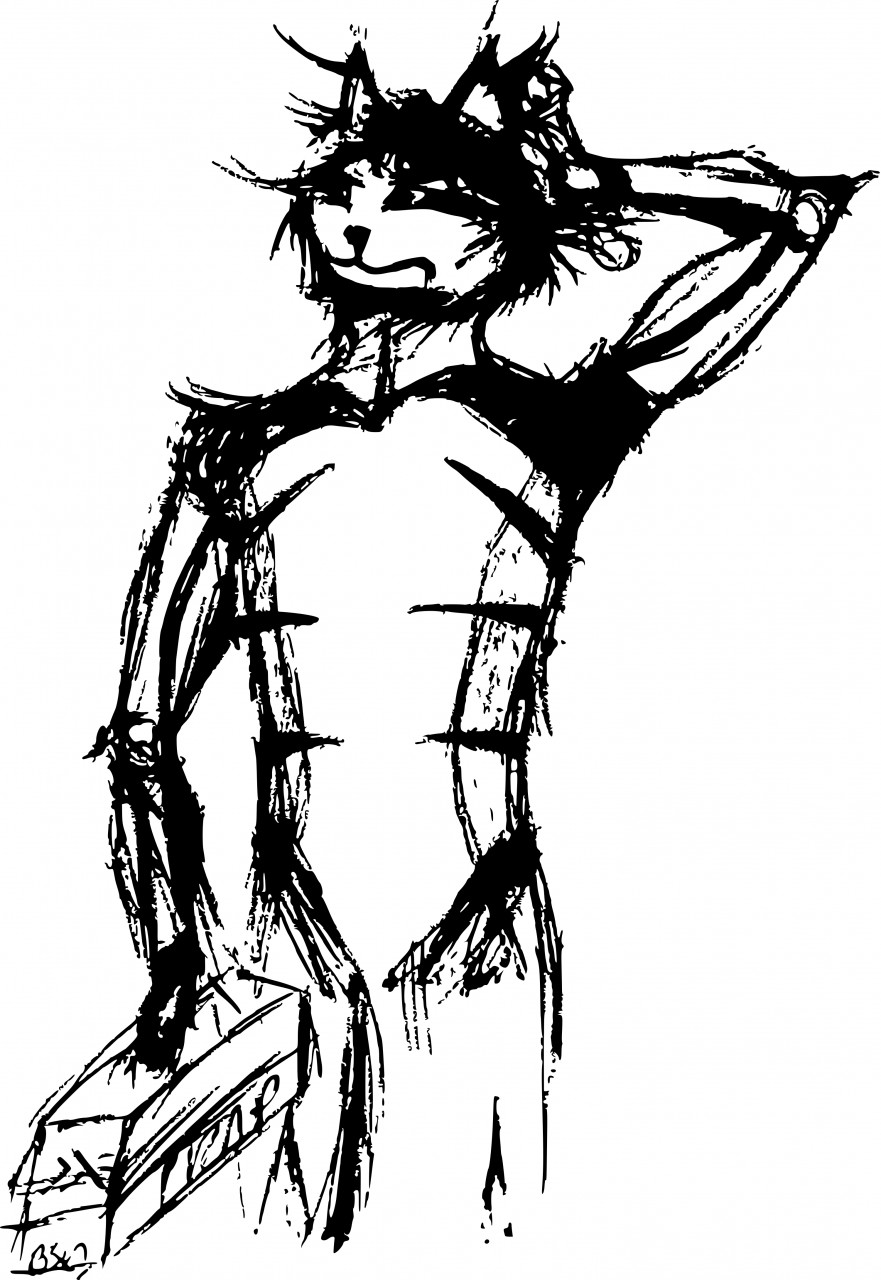
\includegraphics[height=\imageheight]{50x/toolbox/s1v1.jpg}
	\caption[center]{le pamoi versiio be la'o gy.\ WESTERNUNIONSOFTHECOUNTRYWESTERNS .gy}
\end{figure}
\subsection{le remoi tsautu}
.ni'o le remoi tsautu be la'o gy.\ WESTERNUNIONSOFTHECOUNTRYWESTERNS .gy cu pamoi lo'i milxe xamgu pinsi bo tsautu\sds  .i ku'i ti poi tsautu cu .uaigri le vektori pixra poi kibzva la'o gy.\ \url{https://github.com/varikvalefor/drawingstuff/blob/master/50x/toolbox/toolboxsketch002.svg} .gy

\begin{figure}[ht]
	\centering
	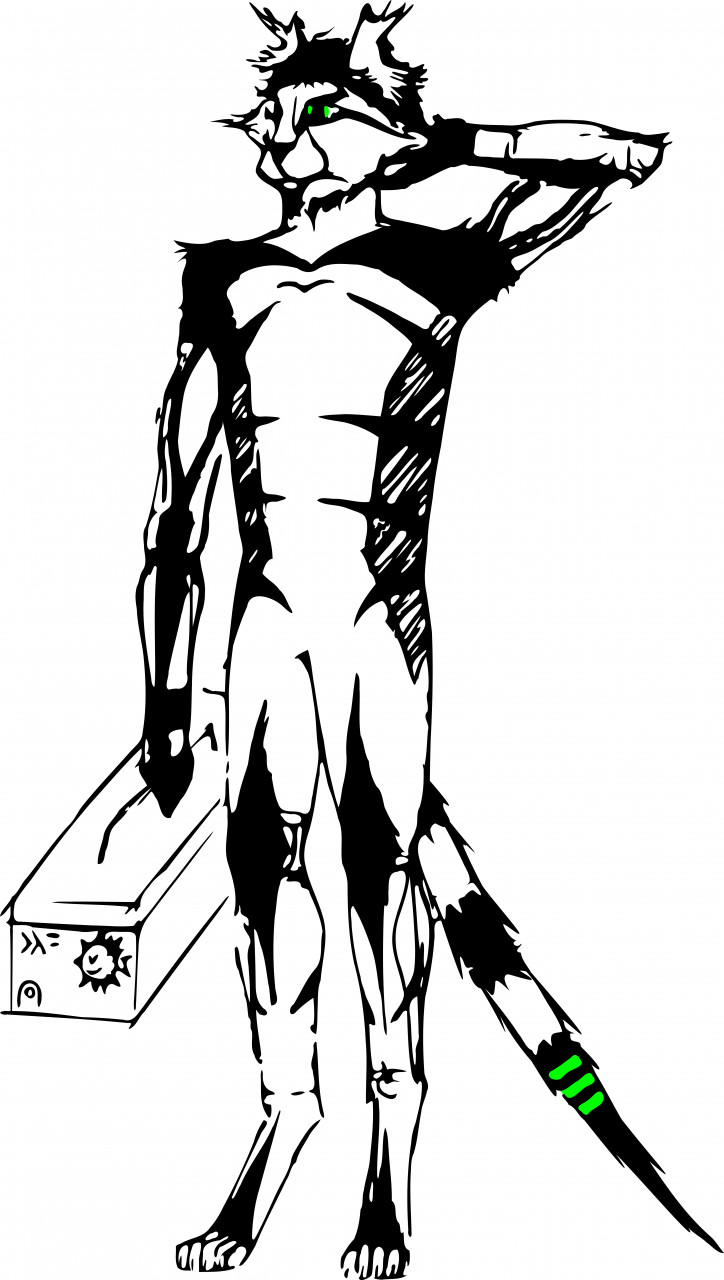
\includegraphics[height=\imageheight]{50x/toolbox/s1v2.jpg}
	\caption[center]{le remoi tsautu be la'o gy.\ WESTERNUNIONSOFTHECOUNTRYWESTERNS .gy}
\end{figure}
\chapter{la'o gy.\ HOLLYWOODFREAKSONTHEHOLLYWOODSCENE .gy}
\begin{figure}[ht]
	\centering
	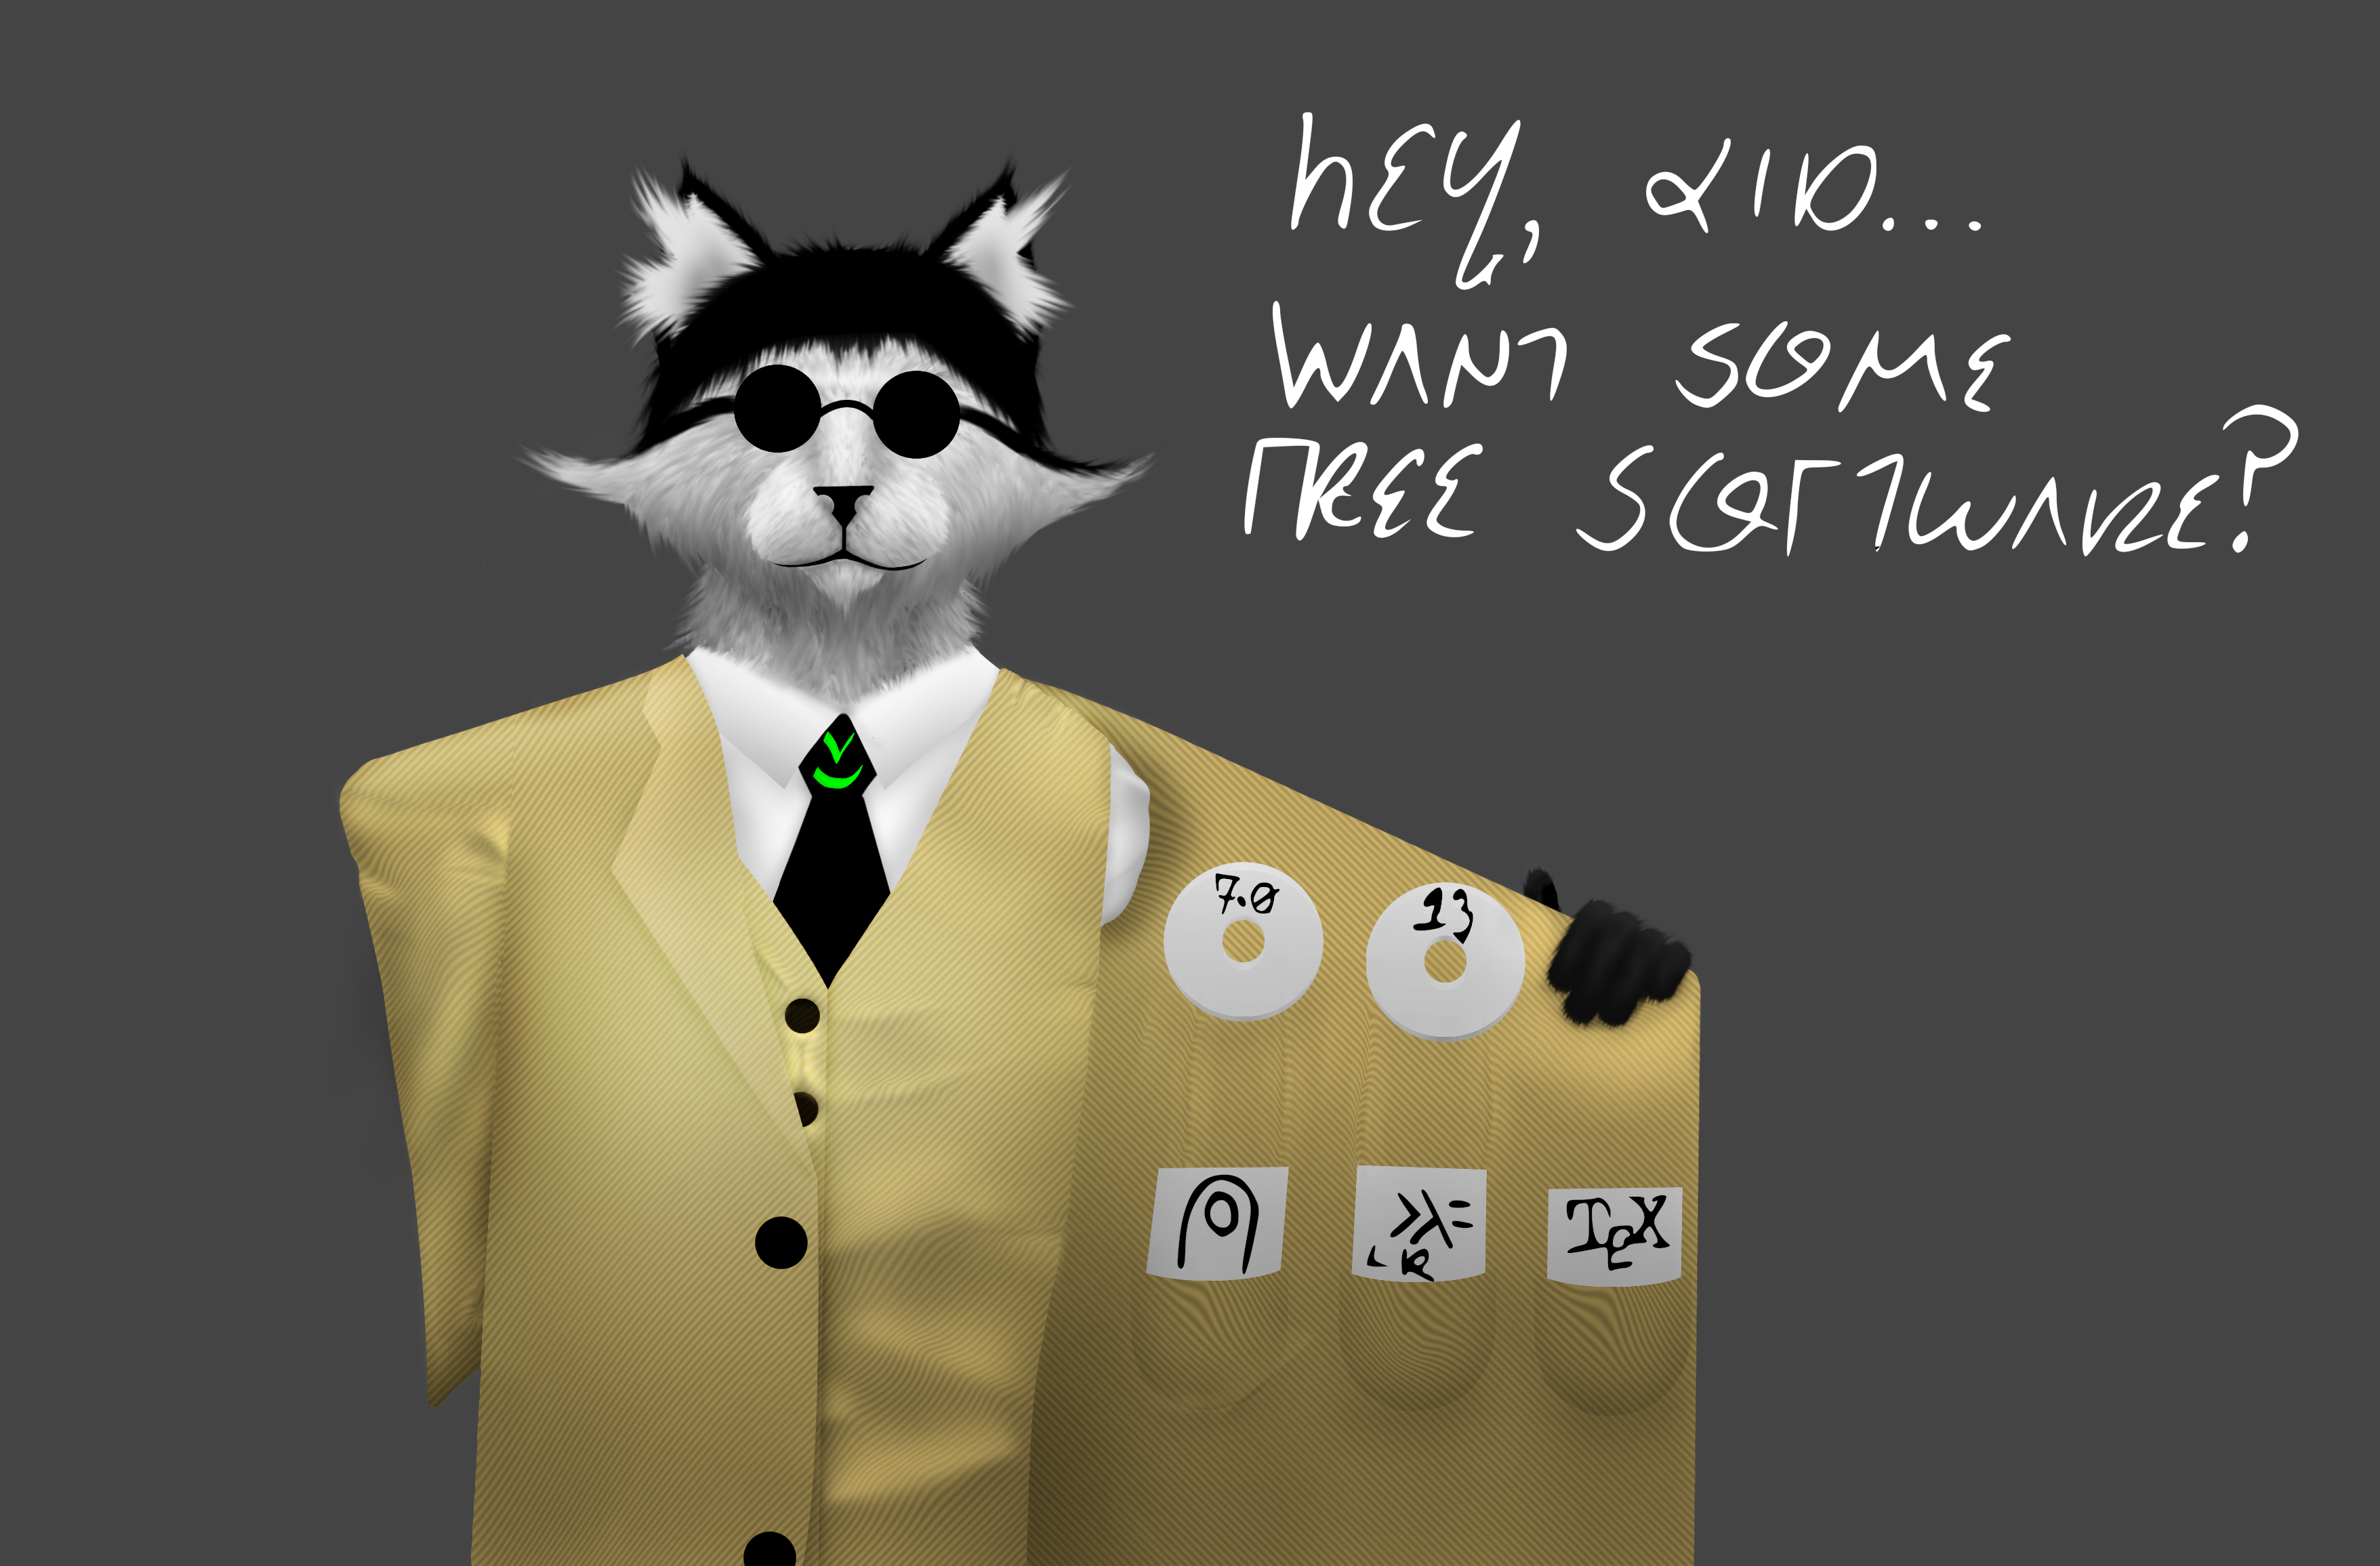
\includegraphics[height=\imageheight]{hollywoodfreaksonthehollywoodscene/hollywoodfreaksonthehollywoodscene.png}
	\caption[center]{la'o gy.\ HOLLYWOODFREAKSONTHEHOLLYWOODSCENE .gy}
\end{figure}
\section{le pamoi velski be le pixra}
\subsection{le bebna ba'e tordu lisri}
.ni'o le ctemidju cu tcika le nu lo prenu goi ko'a cadzu lo klaji\sds  .ije ko'a jibni lo dikca fatri dinju\sds  .ije le prenu poi se viska lo tcidu ku'o goi ko'e klama ko'a lo cmatricu

.i ko'a simlu le ka selspaji\sds  .ije ko'e tcuskuue lu doi le verba\sds  .i xu do djica lo fingubni proga li'u

.i le tcidu cu kakne le nu jivbi'o le du'u fitytu'i gi'a na fitytu'i

\subsection{la'o gy.\ Blah .gy}
.ni'o gubgau le bebna selxamsku

.ni'o ti poi pixra cu bebna selxamsku gi'e pamoi jetnu ju'anai bo troci be le nu la .varik.\ terxra lo bukpu

\subsection{le daski se vasru}
.ni'o le cukmirvelvei poi se tcita zoi gy.\ 7.0 .gy cu cukmirvelvei la'o gy.\ OpenBSD .gy\sds  .i le cukmirvelvei poi se tcita zoi gy.\ 13 .gy cukmirvelvei la'o gy.\ FreeBSD .gy

\subsubsection{le cuktermai}
.ni'o la .varik.\ djica le nu le pixra cu sitna le ziljmina proga kei ca'o le nu la .varik.\ zbasu fo'a\sds  .i da poi sidbo zo'u da na temsepcau mulno pe'a

\subsubsection{le kosta daski}
.ni'o le tcidu cu sruma le du'u le daski cu vasru le papri poi krati pe'a lo te samrkompli po le sambau poi se pilno la .varik.

\subsubsection{li ni'e ni co'e}
.ni'o le nu la .varik.\ djica le nu le pixra cu sitna le ziljmina proga cu cabna le nu la .varik.\ zbasu fo'a\sds  .i ku'i da poi sidbo zo'u da na temsepcau mulno pe'a

\subsection{lo cfilyfacki}
.ni'o lo nu cfilyfacki cu roroi zanvi'e

\subsection{le pilno}
.ni'o pilno la'o gy.\ GIMP .gy le nu zbasu ti poi pixra

.ni'o pilno la'o gy.\ ed(1) .gy le nu ciska dei

\section{le cfila be le pixra}
su'o le prenu poi na me la .varik.\ cu facki le du'u le taxfu poi se pixra la'oi .HOLLYWOODFREAKSONTHEHOLLYWOODSCENE.\ goi ko'a cu smimlu lo pelji

.ni'o si'a la .varik.\ facki le du'u le cukmirvelvei poi se pixra ko'a cu smimlu lo pelji

\subsection{le taxfu poi claxu le ci cimde pe'a}
.ni'o lo so'o prenu cu xusra le du'u le taxfu be la'o gy.\ VUNC .gy ku'o poi se vasru la'o gy.\ HOLLYWOODFREAKSONTHEHOLLYWOODSCENE .gy cu claxu le ci cimde pe'a gi'e smimlu lo pelji .a zo'e

.i la .varik.\ tugni fi le he famsku

.i .o'u le nu dasni lo veljmina be lo pelji kista .e lo pelji nercreka .e lo pelji creka vu'o poi claxu lo trixe cu mutce xajmi

\subsection{le ctino po le cukmirvelvei}
.i la .varik.\ jinvi le du'u le velvei cu tamsmi lo pelji .e lo narcukmirvelvei\sds  .i cumki fa le nu le nabmi cu se rinka le ka le velvei cu tcenarkli

\chapter{la'o gy.\ BROKEDOWNOUTINADITCHOFOLDRUBBISH .gy}
\begin{figure}[ht]
	\centering
	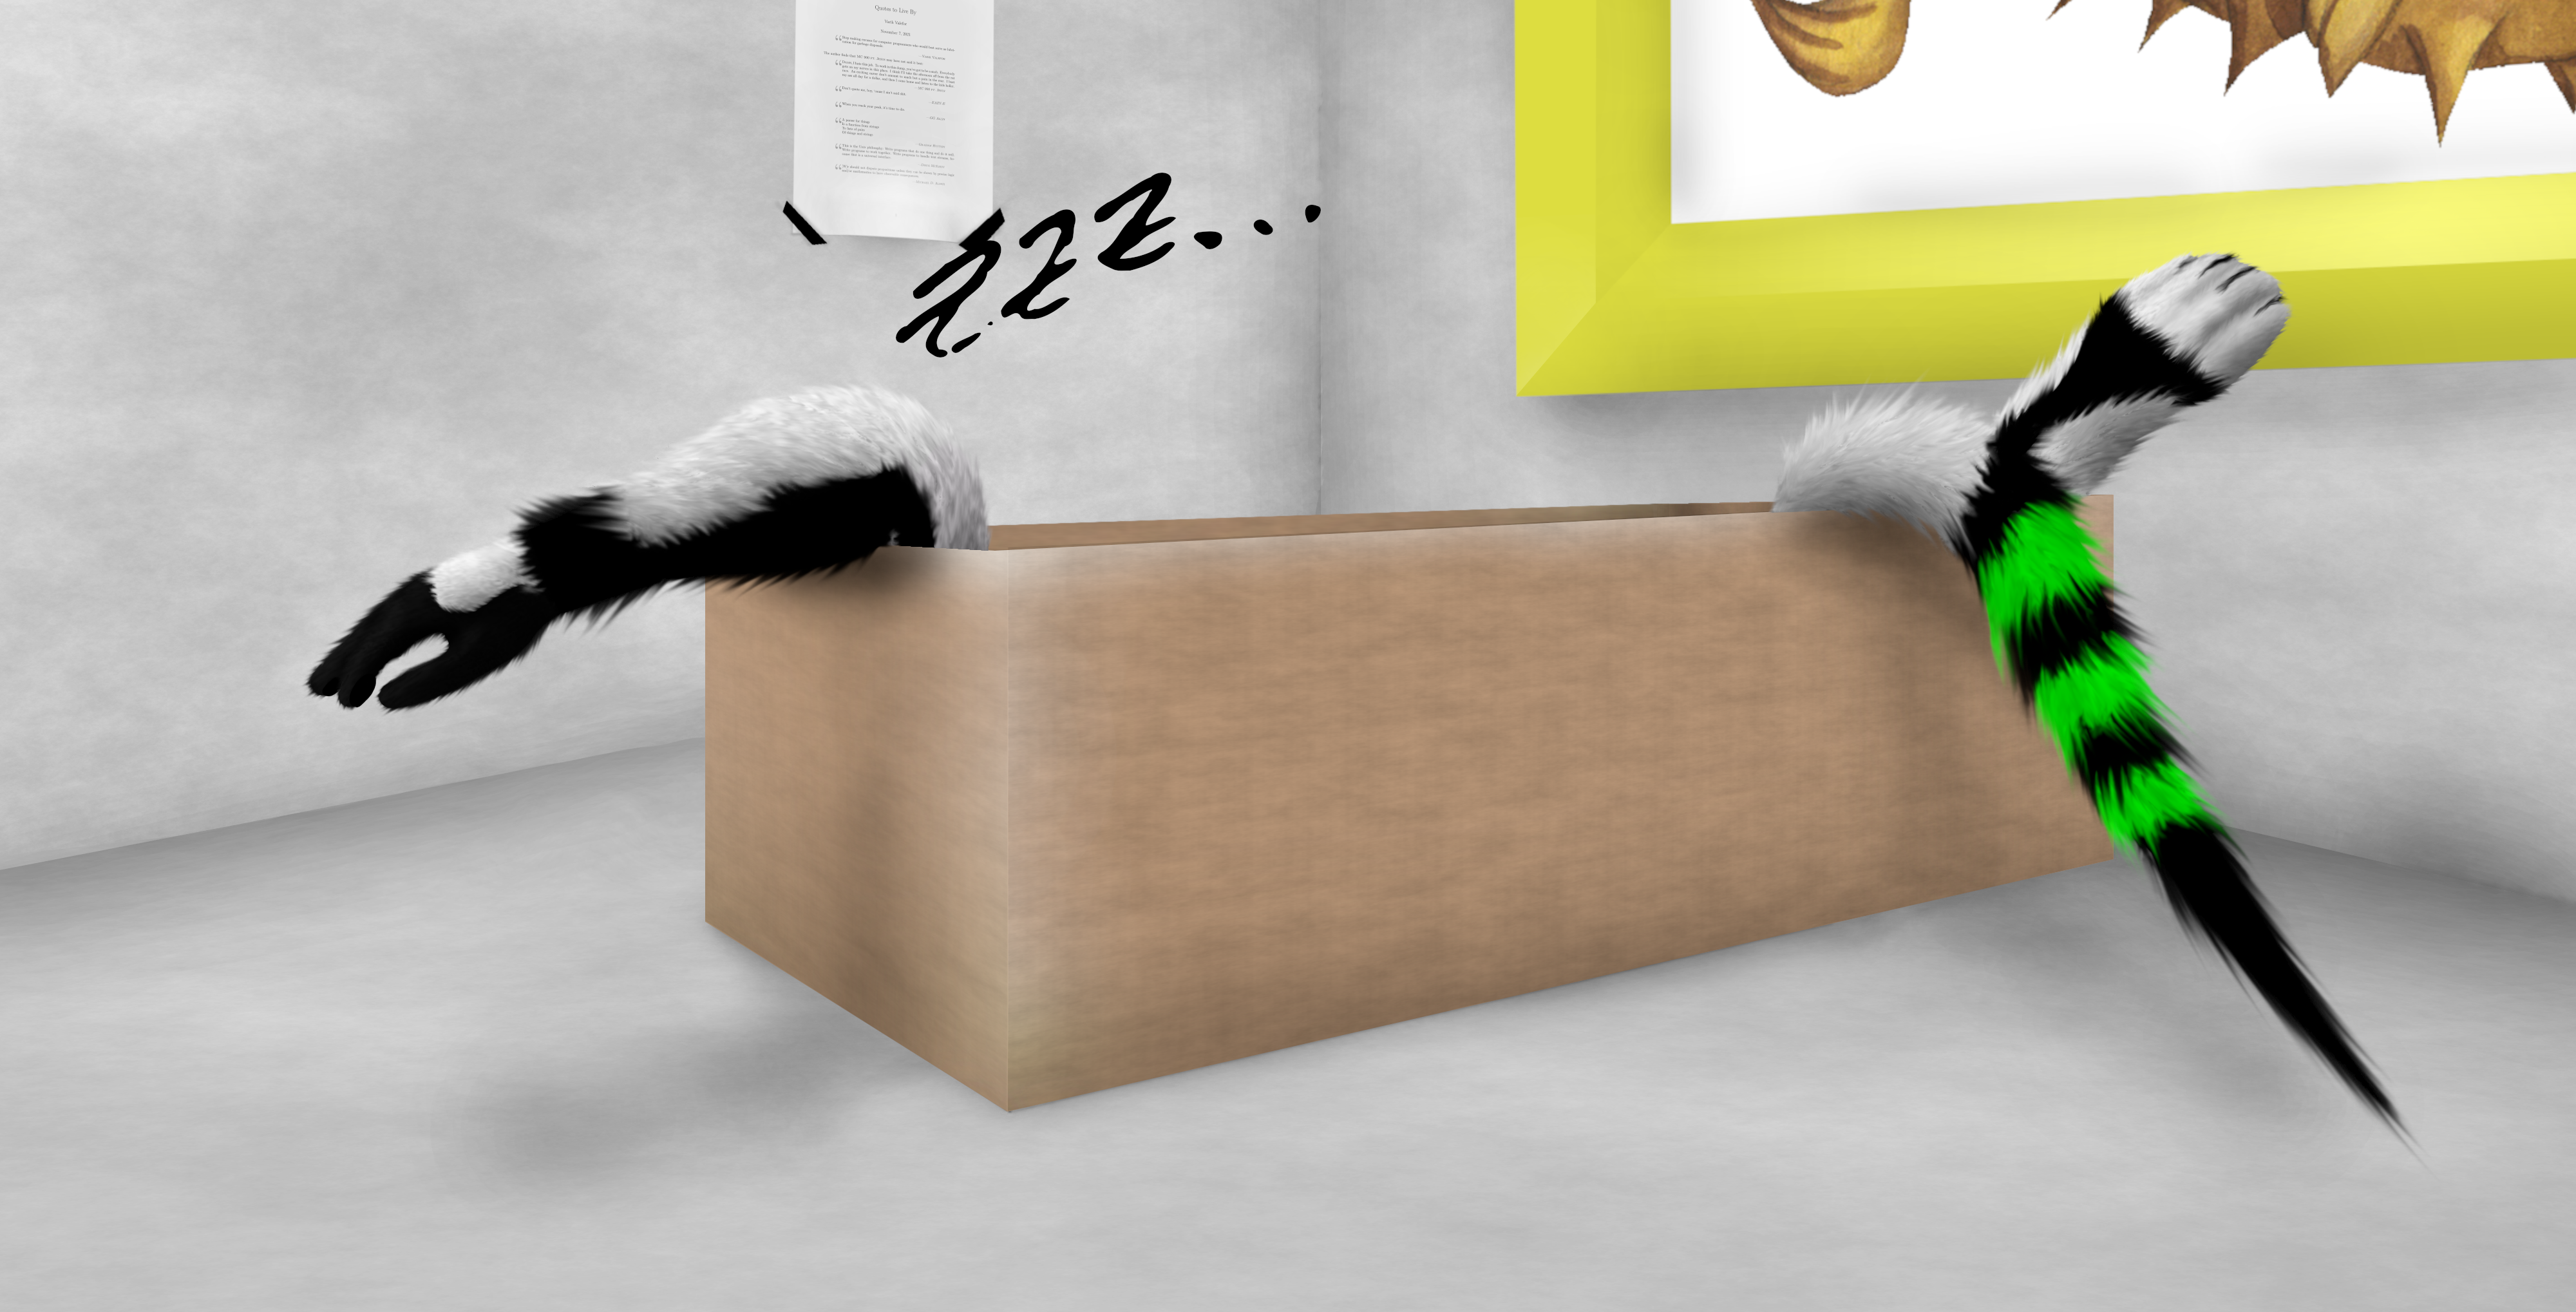
\includegraphics[width=\textwidth]{brokedownoutinaditchofoldrubbish/brokedownoutinaditchofoldrubbish.png}
	\caption[center]{.i ti poi pixra cu du le pixra\sds  .i xu zo'e poi kacmyxra lo xajnuj cu se kanpe\sds  .i doi bebna ko na bebna}
\end{figure}
\section{le pamoi velski be le pixra}
.ni'o lo cnino pixra cu gubni

\subsection{le jetnu pe'a trixe pixra\ldots e lo xamsku}
.ni'o ti poi pixra gi'e se cmene zoi gy.\ BROKEDOWNOUTINADITCHOFOLDRUBBISH .gy cu pamoi lo gubni pixra be fi la .varik.\ ku poi ckaji lo jetnu pe'a trixe pixra .e no lo stodi zilska .e no lo sucta\sds  .i ji'a zoi gy.\ BROKEDOWNOUTINADITCHOFOLDRUBBISH .gy vasru lo so'u xamsku

\subsection{le tanxe}
.ni'o le tcidu cumki sruma le du'u le tinsypleta'e poi vasru le xarpre poi zutse cu tsagau gi'e na se marxa lo cmalu junta\sds  .i ji'a le tcidu cu cumki sruma le du'u le vorme pe'a po le tanxe cu se vasru le tanxe gi'a se vimcu

\subsection{lo se vasru pe'a xamsku}
.ni'o le pamoi versiio be ti poi pixra cu se vasru pe'a xamsku\sds  .i ciska le se vasru pe'a xamsku le tanxe\sds  .i ku'i la .varik.\ pu .uaigri jivbi'o le du'u le se vasru pe'a xamsku cu na mutce xajmi kei gi'e vimcu le se vasru pe'a xamsku

\subsection{zoi gy.\ ZZZ .gy}
.ni'o le nu zoi gy.\ ZZZ .gy se pixra cu .indika le du'u le xarpre cu sipsavgau\sds  .i le nu le xarpre cu sipsavgau kei .indika le du'u le xarpre sipna\sds  .i ku'i zoi gy.\ ZZZ .gy kampu sipsav bo krati ki'u ma

\subsection{lo nu nitpiki}
.ni'o lo nu nitpiki cu za'o se nelci

\subsection{le se cuxna xarci pe'a}
.ni'o pilno la'o gy.\ GIMP .gy le nu zbasu ti poi pixra\sds  .i pilno lo xance degji .ualdo le jetnu pe'a pixra bo gunka

.ni'o pilno la'o gy.\ ed(1) .gy le nu ciska dei

.ni'o la'o gy.\ GIMP .gy .e la'o gy.\ ed(1) .gy bajra pe'a la'o gy.\ OpenBSD .gy

\chapter{la'o gy.\ DANCINGONTHEROOFSHOOTINGHOLESINTHEMOON .gy}
\begin{figure}[ht]
	\centering
	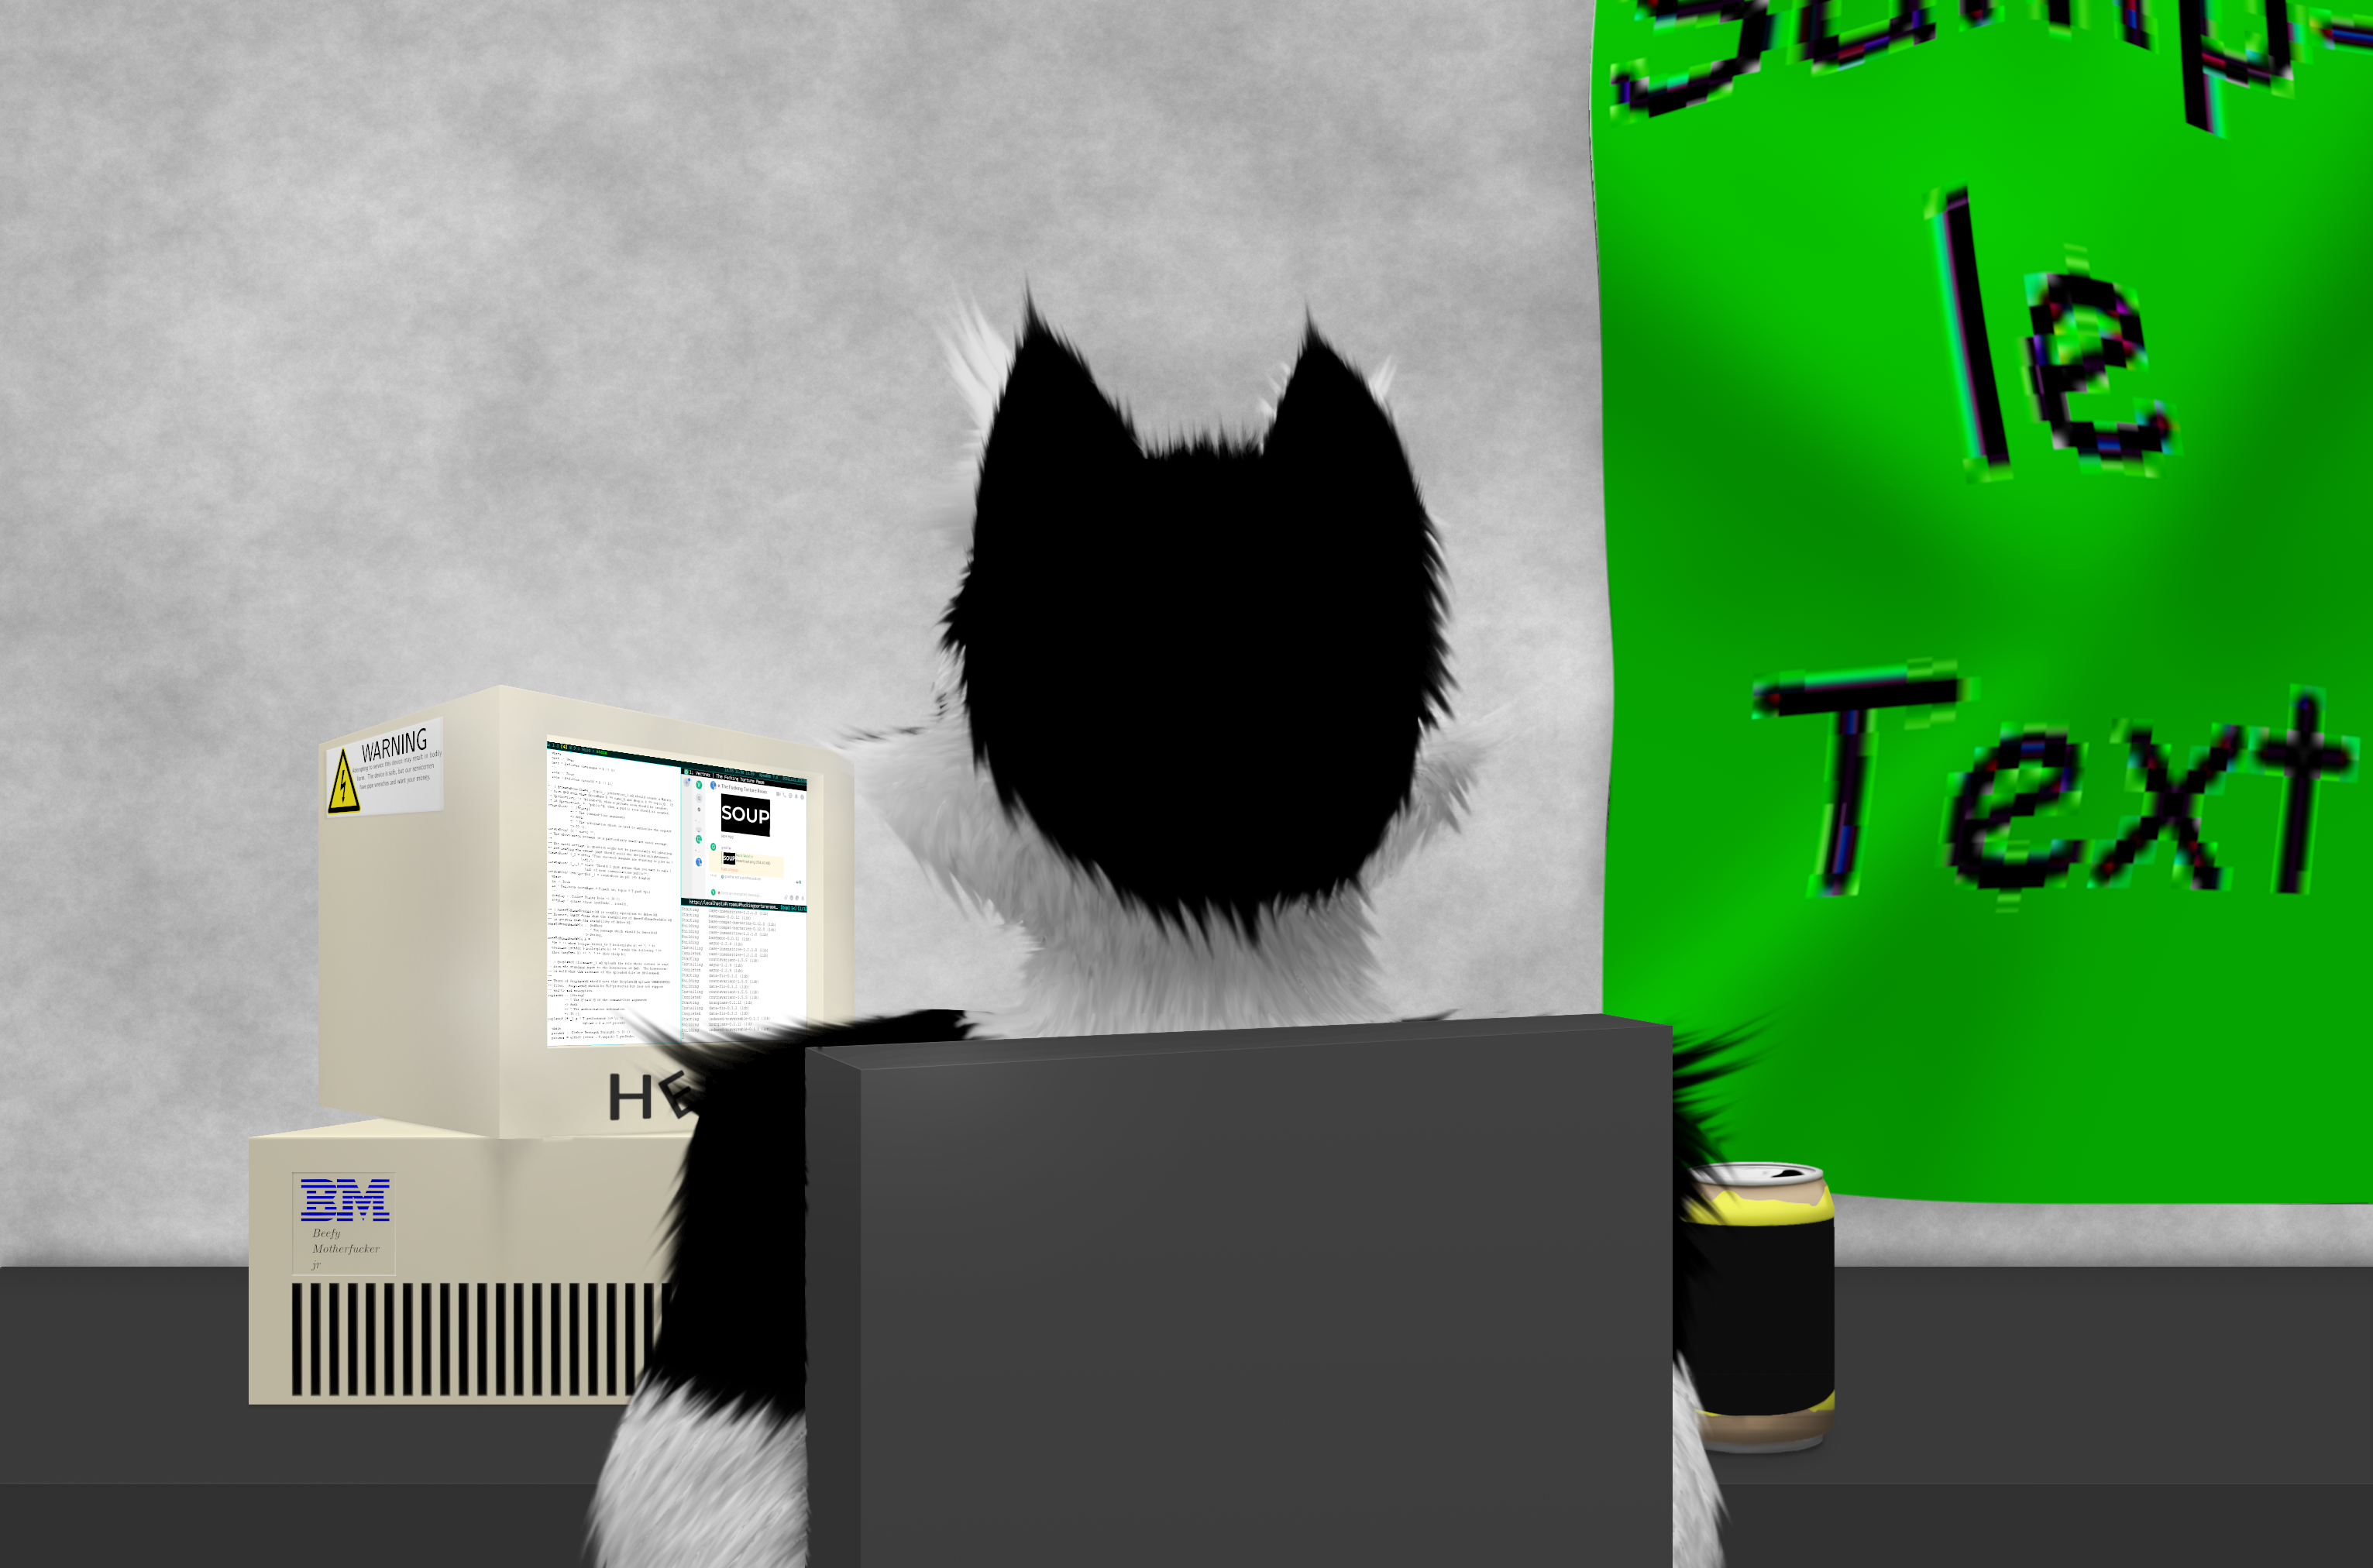
\includegraphics[width=\textwidth]{dancingontheroofshootingholesinthemoon/dancingontheroofshootingholesinthemoon.png}
	\caption[center]{.ni'o le mulbi'o versiio be la'o gy.\ DANCINGONTHEROOFSHOOTINGHOLESONTHEMOON .gy\sds  .ni'o le nu viska lo ro tcila cu frili zo'e le nu pilno lo banro blaci\ldots a lo cmactatci}
\end{figure}
\section{le pamoi velski be le pixra}
.ni'o .ue'i lo ziljmina pixra cu gubni

.ni'o le pixra cu pixra lo roldje tcini\sds  .i ku'i sorpa'a le nu le pixra cu na mutce tolzdi

\subsection{le vlavelski}
zoi gy.\ VUNC .gy krati le xarpre be la .varik.
\subsection{le torveki}
.ni'o ti poi pixra cu pixra le nu la'o gy.\ VUNC .gy jibni gi'e galfi lo proga\ldots gi'e tcidu lo xlali kibzva bo notci kei

\subsection{le selxamsku .e zo'e}
.ni'o le pixra cu simsa le da'a pixra be fi la .varik.\ li ni'e ni se vasru selxamsku\sds  .i le tcidu cumki ciksi le xamsku\sds  .i ku'i ji'a ti poi pixra cu vasru le cmalu jikske bo ckipinka\sds  .i ji'a le tcidu cu cumki skicu le cmalu jikske bo ckipinka

\subsection{zoi gy.\ SOUP .gy}
.ni'o zoi gy.\ SOUP .gy poi simlu lo bebna cu zvati ki'u le nu la .varik.\ na djuno le du'u selfladra le nu le pixra cu zifre vasru le pamoi kacmyxra\sds  .i le nu na te nunflapai la .varik.\ cu frili la .varik.\ le nu le velski pe'a be le kacmyxra cu basti le pamoi kacmyxra

.ni'o zo velski cu sidysmu ki'u le velski pe'a cu na mutce skicu\sds  .i lo zenba velski velski be le pamoi kacmyxra cu du lo'u lo tcesedemri'a kacmyxra be lo kabri poi se vasru lo .alfabeta stasu le'u

\subsection{le kadje tcita}
.ni'o le se tcidu po le kadje tcita cu du zoi gy.
\begin{quote}
	WARNING

	Attempting to service this device may result in bodily harm.\  The device is safe, but our servicemen have pipe wrenches and want your money.
\end{quote}
.gy

\subsection{le batkyfoi}
.ni'o le pixra cu pixra le nu la'o gy.\ VUNC .gy pilno le batkyfoi\sds  .i ku'i le batkyfoi naseviska\sds  .i ku'i je se cumki le nu le du'u la'o gy.\ VUNC .gy pilno le batkyfoi kei zenba xamgu se .indika

\subsection{le nu nitpiki}
.ni'o lo nu nitpiki cu za'o se nelci

\subsection{le plijaspu}
.ni'o ti poi pixra cu selxrapra gi'e selplijaspu la'o gy.\ CC BY-NC 4.0 .gy\sds .i le mulno tcidu po ti poi selplijaspu cu xabju pe'a la'o gy.\ https://creativecommons.org/licenses/by-nc/4.0/legalcode .gy

\subsection{le pilno}
.ni'o pilno la'o gy.\ GIMP .gy le nu zbasu ti poi pixra\sds  .i la'o gy.\ GIMP .gy tcexla\sds  .i ku'i za'a la'o gy.\ GIMP .gy traji le ka ce'u xamgu pixra bo fingubni bo proga

.ni'o pilno la'o gy.\ ed(1) .gy le nu zbasu dei

.ni'o la'o gy.\ GIMP .gy .e la'o gy.\ ed(1) .gy bajra pe'a la'o gy.\ OpenBSD .gy

\section{le cfila be le pixra}
.ni'o le stizu poi selzutse la'oi .VUNC.\ cu claxu lo tcila

\subsection{le stizu}
.ni'o le nu le stizu poi selzutse la'o gy.\ VUNC .gy cu claxu lo tcila cu se rinka le nu le stizu tengu cu .ambigu'o\sds  .i le stizu se.enge cu selstaile\sds  .i la .varik.\ mutce nelci lo dijyzbaske po la'o gy.\ Brutalism .gy\sds  .i ku'i krici le du'u le stizu cu mabla

\chapter{la'o gy.\ ITHINKWEREGOINGCRAZY .gy}
\begin{figure}[ht]
	\centering
	\includegraphics[height=10cm]{ithinkweregoingcrazy/ithinkweregoingcrazy.png}
	\caption[center]{la'o gy.\ ITHINKWEREGOINGCRAZY .gy}
\end{figure}
\section{The Original Description of the Drawing}
.ni'o zoi gy.\ BLOCKED BY SHODAN LEVEL SECURITY .gy

\subsection{lu mi viska ma li'u}
.ni'o ti poi pixra cu pixra le nu le xarpre be la .varik.\ smimlu la'o gy.\ SHODAN .gy po la'o gy.\ \textit{System Shock} .gy le ka jorne lo jimsko kei .e le ka selnunfirsku fi lo nutli

\subsection{le tcika}
.ni'o ji'i za'a le pavrelmasti cu vasru pe'a lo su'o pa pixra

\subsection{le citri}
\subsubsection{le tsautu}
.ni'o lo pamuki'oki'o nanca cu se puvza le nu la .varik.\ gubni le tsautu poi pixra le nu la'o gy.\ VUNC .gy simlu la'o gy.\ SHODAN .gy po la'o gy.\ \textit{System Shock} .gy le ke jorne lo jimsko

\subsubsection{le pamoi se troci se galfi}
.ni'o la .varik.\ tolsti le nu galfi le tsautu lo jetnu pe'a pixra\sds  .i ku'i le nu la .varik.\ zbasu lo nurfu'i cu se purci snuti vimcu le datni be le cukmakyvelvei po le ralju skami po la .varik.\sds  .i ja'e le pamoi versiio be le pixra cu lakne cimni bo farcri pe'a

\subsubsection{le remoi se troci se galfi}
.ni'o li papa pi'e vo pi'e renorepa cu detri le nu la .varik.\ tolsti le nu galfi le tsautu lo jetnu pe'a pixra gi'e jmina lo tsautu poi nasevasru loi sirsunla lo samrxra be fi la'o gy.\ Scalable Vector Graphics .gy\sds  .i snada le nu mulno le pruce

\subsubsection{le nu troci le nu jmina lo tcila}
.ni'o li ji'i re pi'e xa pi'e renorepa cu detri le nu la .varik.\ galfi le samrxra be fi la'o gy.\ Scalable Vector Graphics .gy lo samrxra be fi la'o gy.\ XCF .gy gi'e tolsti le nu jmina lo tcila\sds  .i le nu jmina lo tcila cu lidne le nu jmina lo jimsko kei ki'u zo'e

.ni'o lo jetnu pe'a nabmi ku sotmei\sds  .i ku'i la .varik.\ nanelci le jalge be le nu jmina le tcila kei gi'e zasysti le nu zbasu le pixra

\subsubsection{le nu se snada jmina bo tcila}
.ni'o li reze pi'e papa pi'e renorepa cu detki le nu la .varik.\ to'ezasysti le nu zbasu le pixra gi'e ku'i ninke'u jivbi'o le du'u la'o gy.\ GIMP .gy cumki kalci\ldots pe'a

\subsubsection{le nu mulgau le pixra}
.ni'o li pa pi'e pare pi'e renorepa cu detni le nu la .varik.\ xusra le du'u le pixra cu selmulgau

\subsection{le nu le ti poi pixra cu te gumgau}
.ni'o ko'a goi la'o gy.\ SHODAN .gy po la'o gy.\ \textit{System Shock} .gy velfi'i le pagbu be le pixra ku poi se finti fo ko'a\sds  .i ku'i le nu la .varik.\ napilno lo pa versiio be ko'a cu cabna le nu la .varik.\ zbasu ti poi pixra\sds  .i lo menli gumgau be ko'a po la'o gy.\ \textit{System Shock} .gy .e ko'a po la'o gy.\ \textit{System Shock 2} .gy cu velfi'i ti poi pixra ku'o fo la .varik.
\subsection{lo nu nitpiki}
.ni'o lo nu nitpiki cu za'o se nelci

\subsection{le plijaspu}
.ni'o ti poi pixra cu selxrapra gi'e selplijaspu la'o gy.\ CC BY-NC 4.0 .gy\sds  .i le mulno tcidu po ti poi selplijaspu cu xabju pe'a la'o gy.\ https://creativecommons.org/licenses/by-nc/4.0/legalcode .gy

\subsection{le pilno}
.ni'o pilno la'o gy.\ GIMP .gy le nu majgau ti poi pixra\sds  .i  la'o gy.\ GIMP .gy xlatce\sds  .i ku'i zmanei la'o gy.\ GIMP .gy la'o gy.\ Krita .gy

.ni'o i ciska dei fo la'o gy.\ ed(1) .gy

.ni'o la'o gy.\ GIMP .gy .e la'o gy.\ ed(1) .gy bajra pe'a la'o gy.\ OpenBSD .gy

\section{le kanla se cortu}
.ni'o so'u da poi prenu zo'u da xusra le du'u le nu da catlu la'o gy.\ ITHINKWEREGOINGCRAZY .gy kei cu se jalge le nu da cortu kei kei goi ko'a\sds  .i la .varik.\ jijyji'i le du'u lo prenu poi xusra ko'a cu du'eski ko'a gi'a bilma lo kanla se cortu kei ki'u le nu la .varik.\ na zatfa'i lo satci krasi be le kanla se cortu

\section{le se frati}
.ni'o le nu la'o gy.\ ITHINKWEREGOINGCRAZY .gy nasopnelsei\ldots cu cumki se krinu le nu zo'e poi velfi'i la'o gy.\ ITHINKWEREGOINGCRAZY .gy rirci

\subsection{le velski be le se frati}
.ni'o su'o da poi pixra fi la .varik.\ zo'u li ni'e ni lo prenu cu nelci la'o gy.\ ITHINKWEREGOINGCRAZY .gy cu dubme'a li ni'e ni lo prenu cu nelci da

\subsection{le cumki rinka be le narselnei}
.ni'o la .varik.\ jinvi le du'u le narselnei po la'o gy.\ ITHINKWEREGOINGCRAZY .gy  cu cumki se krinu le nu zo'e poi velfi'i la'o gy.\ ITHINKWEREGOINGCRAZY .gy rirci

\begin{thm}
.ni'o se lakne le du'u lo so'u prenu cu nelci la'o gy.\ ITHINKWEREGOINGCRAZY .gy

\end{thm}
\begin{proof}
${}$
.ni'o ro da zo'u ro de poi pixra zo'u ro di poi prenu zo'u le du'u de velsitsku da cu nibyti'i le du'u di mulsmujmi de nagi'a se slabu de

.ni'o ro da poi pixra zo'u le du'u lo so'u prenu ku mulsmujmi da cu nibyti'i le du'u se lakne le du'u lo so'u prenu ku nelci da\footnote{.ni'o le tcidu cu se darsygau milxe bo senpi ti poi pixra}

.ni'o so'u prenu cu slabu la'o gy.\ \textit{System Shock} .gy\footnote{.ni'o zo so'u cumki dukse bo ruble}

.ni'o la'o gy.\ ITHINKWEREGOINGCRAZY .gy velsitsku la'o gy.\ \textit{System Shock} .gy

.ni'o ja'e se lakne le du'u lo so'u prenu cu nelci la'o gy.\ ITHINKWEREGOINGCRAZY .gy

\end{proof}
\chapter{la'o gy.\ JUDASTRAINWRECK .gy}
\begin{figure}[ht]
	\centering
	
\includegraphics[height=10cm]{judastrainwreck/judastrainwreck.png}
	\caption[center]{la'o gy.\ JUDASTRAINWRECK .gy}
\end{figure}
\section{le pamoi velski be ti poi pixra}
la .varik.\ jinvi le du'u le firxa'e cu melbi

\subsection{le torveki}
.ni'o su'o da poi papri bo pixra tsautu zo'u da binxo le vektori pixra poi binxo ti poi pixra

.ni'o le tcidu tanxe pe'a vasru lo toltce bo galfi notci poi pu selterbe'i la .varik.

.ni'o ti poi pixra cu selxrapra gi'e selplijaspu la'o gy.\ CC BY-NC 4.0 .gy

.ni'o doi la'o gy.\ lamer .gy ko pilno la'o gy.\ OpenBSD .gy

\subsection{le pruce poi gasnu le nu le tsautu ku binxo le mulno pixra}
.ni'o la .varik.\ majgau le pamoi tsautu ki'u le nu la .varik.\ djica le nu la .varik.\ terxra lo nasteci

.i la .varik.\ gasnu le nu le pamoi tsautu cu binxo le vektori pixra ki'u le nu la .varik.\ djica le nu la .varik.\ terxra zo'e poi trina

.i le nu la .varik.\ terxra le cabna pixra cu milxe se krinu le nu la .varik.\ djica le nu la .varik.\ ckasu lo prenu poi cusku lo bebna preti.\ gi'a bebna pensi

\subsection{le tcidu tanxe pe'a}
.ni'o le tcidu tanxe pe'a vasru lo toltce bo galfi notci poi pu selterbe'i la .varik.

.i le nu la .varik.\ fuktra la'o gy.\ SIDESHOW BOB .gy le nu cmoni cu se balvi le nu la .varik.\ jdice le du'u le nu la .varik.\ ckasu le prenu gi'e curmi le nu le prenu ku cmecau cu filri'a le nu cmila

\subsection{le plijaspu}
.ni'o ti poi pixra cu selxrapra gi'e selplijaspu la'o gy.\ CC BY-NC 4.0 .gy\sds  .i le mulno tcidu po ti poi selplijaspu cu xabju pe'a la'o gy.\ https://creativecommons.org/licenses/by-nc/4.0/legalcode .gy

\subsection{le pilno}
.ni'o pilno la'o gy.\ GIMP .gy le nu majgau ti poi pixra\sds  .i  la'o gy.\ GIMP .gy xlatce\sds  .i ku'i zmanei la'o gy.\ GIMP .gy la'o gy.\ Krita .gy

.ni'o ciska dei fo la'o gy.\ ed(1) .gy

.ni'o la'o gy.\ GIMP .gy .e la'o gy.\ ed(1) .gy bajra pe'a la'o gy.\ OpenBSD .gy

\section{le selji'i be fi la'o gy.\ JUDASTRAINWRECK .gy}
.ni'o so'u lo prenu cu gubni nitpiki la'o gy.\ JUDASTRAINWRECK .gy\ldots gi'e gubni zausku la'o gy.\ JUDASTRAINWRECK .gy

\subsection{su'o lo selji'i be fi la'o gy.\ JUDASTRAINWRECK .gy}
.ni'o su'o le selji'i be fi la'o gy.\ JUDASTRAINWRECK .gy goi ko'a cu cnita dei

\begin{itemize}
	\item .i ko'a .indika le du'u le selxra be fe ko'a ku goi ko'e cu mapra keitci kei ku ri'a le nu ko'a .indika le du'u le kerfa be fe ko'e cu dukse 
	\begin{itemize}
		\item .i ku'i la .varik.\ toltu'i zo'e le du'u go'i
	\end{itemize}
	\item .i ko'a pixra le .ambigu
	\begin{itemize}
		\item .i la .varik.\ mlitu'i zo'e le du'u go'i
	\end{itemize}
	\item .i ko'a citmle
	\begin{itemize}
		\item .i la .varik.\ no'e tugni zo'e le du'u go'i
	\end{itemize}
\end{itemize}
\section{le ctino}
.ni'o la .varik.\ jinvi le du'u cumki fa le nu li ni'e ni la'o gy.\ JUDASTRAINWRECK .gy goi ko'a vasru le ctino cu dukse kei kei .e le du'u ko'a dukse manku

\section{le xance}
.ni'o la'o gy.\ JUDASTRAINWRECK .gy .indika le du'u le xance degji be fi la'o gy.\ VUNC .gy ku goi ko'a tordu\sds  .i ku'i ko'a na tordu\sds  .i .u'i la'oi .JUDASTRAINWRECK.\ xlali pixra le xance be la'oi .VUNC.

\section{da'a le versiio be la'oi .JUDASTRAINWRECK.}

\subsection{la'o gy.\ JUDASTRAINWRECK-NOHANDLEBARS .gy}
\begin{figure}[ht]
	\centering
	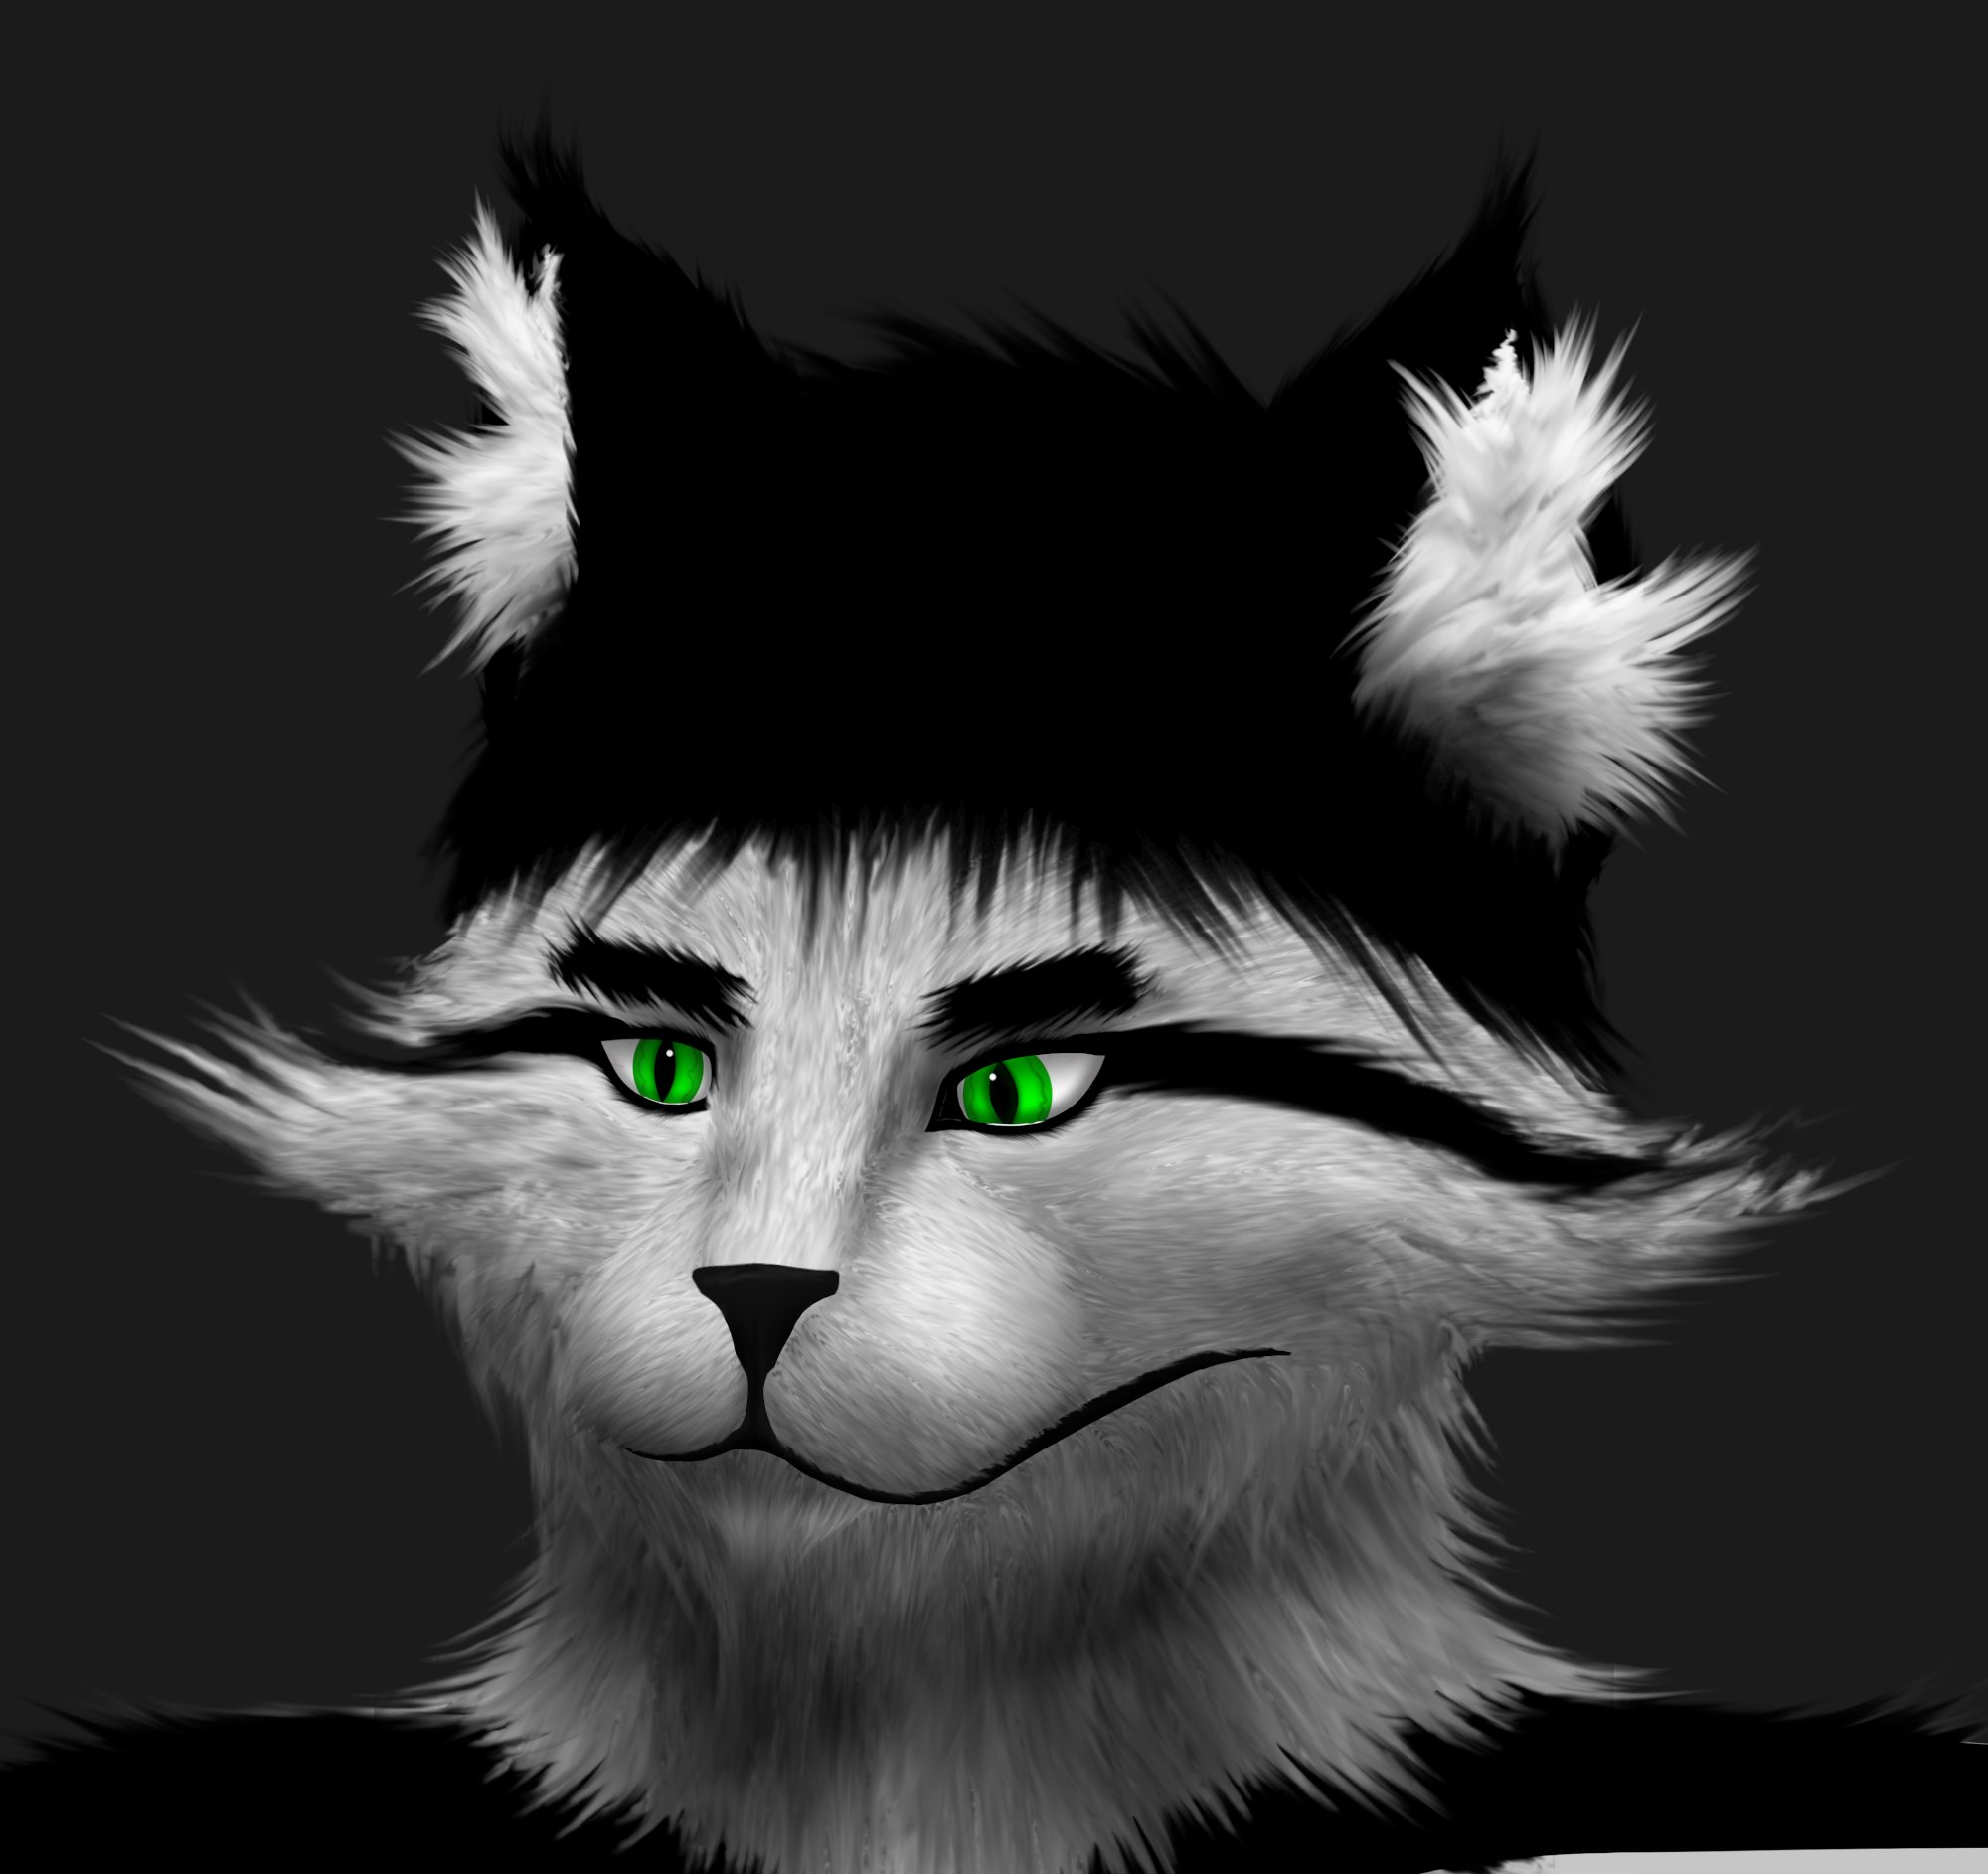
\includegraphics[height=10cm]{judastrainwreck/judastrainwreck-nohandlebars.png}
	\caption[center]{gubgau le versiio be la'oi .JUDASTRAINWRECK.\ ku poi na pixra le birka be la'oi .VUNC.}
\end{figure}
.ni'o la'o gy.\ JUDASTRAINWRECK-NOHANDLEBARS .gy cu versiio la'oi .JUDASTRAINWRECK.\ gi'e na pixra le birka be la'oi .VUNC.

\chapter{la'oi .THROWTHOSEPICTURESDOWNTHELANE.}
\section{le pixra}
\begin{figure}[ht]
	\centering
	\includegraphics[height=\imageheight]{throwthosepicturesdownthelane/throwthosepicturesdownthelane.png}
	\caption[center]{ti poi la'oi .caption.\ cu na vasru lo selxamsku}
\end{figure}
\section{le pamoi velski}
\subsection{le torveki}
la .varik.\ rinka le nu fanmo le nu la .varik.\ zasysti le nu la .varik.\ terxra kei kei kei gi'e gubyternoi .ui le cnino pixra

.ni'o pixra le nu la'oi .VUNC.\ renro la'oi .discus.\ poi cizra gi'e xunre gi'e kinli gi'e te ciska fe la'oi .lambda.\ poi to'alfu

.ni'o la .varik.\ terxra fi ti poi pixra ki'u le nu la .varik.\ djica le nu la .varik.\ salci le nu la .varik.\ tolri'ugau le se zbasu be la .varik\ldots gi'e tervenynoi la'oi .Matel.

.ni'o le nu jmina lo srasu ti poi pixra

.ni'o la'o gy.\ public domain .gy vasru ti poi pixra\ldots .e ro le pixra be fi la .varik.

.ni'o ranji fa le nu la .varik.\ tervencpe lo nu nitpiki

.ni'o la .varik.\ pilno la'oi .GIMP.\ .e la'oi .OpenBSD.\ .e .oiru'e .u'i la'oi .trackpad.

\subsection{le fanmo be le nu zasysti}
le nu la .varik.\ bilma gi'e fliba le nu li renorerepi'enore detri le nu la .varik.\ terxra cu selbalvi le nu la .varik.\ gubyternoi le cnino pixra\sds  .i ti poi cnino pixra cu se cmene zo'oi THROWTHOSEPICTURESDOWNTHELANE

\subsection{le velski be le pixra}
la'oi .THROWTHOSEPICTURESDOWNTHELANE.\ pixra le nu la'oi .VUNC.\ renro la'oi .discus.\ poi ca'a sinxa la'oi .Matel.\ noi samru'e gi'e se zbasu la .varik.\sds  .i lo prenu poi ke'a goi ko'a zo'u cumki fa le nu la'oi .Matel.\ cinri ko'a kei ku ku goi ko'a milxe gleki le nu ko'a djuno le du'u la'oi \url{https://github.com/varikvalefor/matel} zdani pe'a le samselpla po la'oi .Matel.

\subsection{le mukti}
la .varik.\ terxra fi la'oi .THROWTHOSEPICTURESDOWNTHELANE.\ ki'u le nu la .varik.\ djica le nu la .varik.\ salci le nu la .varik.\ renro pe'a la'oi .Matel.\ la'o gy.\ public domain .gy\ldots kei kei .e zo'e

\subsection{le srasu}
ti poi pixra cu pixra le srana .e zo'e\sds  .i rirci fa le nu la .varik.\ terxra fi lo srana

.ni'o la .varik.\ pu zu jmina le srasu ti poi pixra

.ni'o la .varik.\ troci le nu la .varik.\ jmina le srasu ti poi pixra kei le nu la .varik.\ pilno le te galfi fi la .varik.\ fe le tadji be le nu la .varik.\ pixra loi sirsunla kei ku ku ku le nu terxra le srasu ti poi pixra\sds  .i la .varik.\ na mutce jinvi fi le jalge be le nu la .varik.\ pilno le te galfi\ldots ku'i gi'e jinvi le du'u lakne fa le nu le jalge cu tcemlixau

\subsection{la'o gy.\ public domain .gy}
la'oi .THROWTHOSEPICTURESDOWNTHELANE.\ vasru la'o gy.\ public domain .gy gi'e se plijap la'oi .Unlicense.\ noi se skicu la'o gy.\ \url{https://unlicense.org} .gy

.no'i la .varik.\ radji'i le du'u li ni'e ni la'oi .Unlicense.\ mapti lo samru'e kei cu zmadu li ni'e ni la'oi .Unlicense.\ mapti lo pixra\sds  .i ku'i la .varik.\ pilno la'oi .Unlicense.\ ki'u le nu la .varik.\ nelci le nu la'oi .Unlicense.\ tordu kei gi'e to'e nelci le nu la'oi .CC0.\ .e zo'e cu clani

.no'i ji'a ro le pixra poi pu se gubyternoi la .varik.\ cu pu binxo lo se plijap be la'oi .Unlicense.

.no'i ji'a ji'a so'e lo se zbasu be la .varik.\ se renro pe'a fi la'o gy.\ public domain .gy

\subsection{lo nu nitpiki}
la .varik.\ tervencpe lo nu nitpiki ti poi pixra kei ku poi ke'a goi ko'a zo'u cumki fa le nu la .varik.\ pilno ko'a

.no'i si'a la .varik.\ na djica lo nu tcila claxu to'e nitpiki

.no'i lo'i mupli poi ke'a goi ko'a zo'u cumki fa le nu la .varik.\ pilno ko'a cu se vasru lu mi to'e nelci ti li'u noi selfilsmu lu mi to'e nelci le se pixra li'u .e lu mi to'e nelci le pixra li'u

\subsection{le pilno}
uecu'i la .varik.\ pilno la'oi .GIMP.\ .e la'oi .OpenBSD.\ .e .u'i ko'a goi la'oi .trackpad.\ poi mutce milxe mabla ku'o le nu la .varik.\ terxra fi la'oi .THROWTHOSEPICTURESDOWNTHELANE.\sds  .i le nu pilno ko'a le nu terxra cu fi te prali le nu lebna lo xamgu sevzi cusku noi se cinri no lo prenu

\section{le nu cfifa'i poi se zbasu la .varik.}
su'o le'i se cfifa'i be la .varik.\ bei la'oi .THROWTHOSEPICTURESDOWNTHELANE.\ goi ko'a cu se cmima
\begin{itemize}
	\item le du'u la .varik.\ jinvi le du'u le srasu poi se pixra ko'a cu smimlu loi sirsunla kei kei .e
	\item le du'u ko'a pixra le nu le kanla be la'oi .VUNC.\ cu claxu lo tcila
\end{itemize}

\subsection{le ka le srasu poi se pixra cu smimlu loi sirsunla}
la .varik.\ jinvi le du'u le srasu poi se pixra la'oi .THROWTHOSEPICTURESDOWNTHELANE.\ goi ko'a cu smimlu loi sirsunla kei .e le du'u lakne le nu le ka smimlu loi sirsunla cu se rinka le nu le pu'u la .varik.\ terxra le srasu cu smimlu le pu'u la .varik.\ terxra loi sirsunla\sds  .i ku'i la .varik.\ cpedu lo se jinvi be lo prenu poi na me la .varik.\ bei fi le srasu poi se pixra ko'a

\subsection{le du'u ko'a pixra le nu le kanla be la'oi .VUNC.\ cu claxu lo tcila}
la'oi .THROWTHOSEPICTURESDOWNTHELANE.\ goi ko'a vasru pareki'oki'o le vidnysle\ldots gi'e ku'i claxu lo tcila be ro le kanla be la'oi .VUNC.\ ku goi ko'e\sds  .i sa'unai ko'a pixra le nu ko'e claxu lo selvi'a blutu'u .e la'oi .striation.\ pe le kalca'osrumu'a\sds  .i la .varik.\ jinvi le du'u le nu ckaji le ka mo'isti cu te dapma

\section{le nu cfifa'i poi na se zbasu la .varik.}
su'o le prenu cu cfifa'i zo'e la'oi .THROWTHOSEPICTURESDOWNTHELANE.\sds  .i la'edi'u pluka la .varik.\sds  .i le torveki be su'o le nu cfifa'i cu se mupli
\begin{itemize}
	\item lu le birka be la'oi .VUNC.\ cu duske clani li'u .e
	\item lu le loldi cu dukse xekri li'u .e
	\item lu le srasu poi darno le kacma pe'a cu dukse se gusni li'u .e
	\item lu le tuple be la'oi .VUNC.\ cu dukse tordu li'u .e
	\item lu le dizlo zunle kinli be le nercreka pe'a po la'oi .VUNC.\ cu dukse galtu li'u .e
	\item lu dukse viska le zunle tuple be la'oi .VUNC.\ li'u .e
	\item lu le selxra xarpre cu smimlu lo sampre li'u
\end{itemize}

\subsection{lu le birka be la'oi .VUNC.\ cu duske clani li'u}
su'o le prenu cu xusra le du'u le birka be le versiio be la'oi .VUNC.\ ku poi se pixra la'oi .THROWTHOSEPICTURESDOWNTHELANE.\ cu dukse clani kei goi ko'a\sds  .i la .varik.\ milxe tugni fi ko'a\ldots gi'e ku'i jinvi le du'u lakne fa le nu le ka le birka cu clani ku ju'anai jalge le .asna be la'oi .VUNC.\ ku poi se pixra la'oi .THROWTHOSEPICTURESDOWNTHELANE.\ldots kei kei gi'e ku'i je'a radji'i le du'u cumki fa le nu le birka be la'oi .VUNC.\ cu dukse clani

\subsection{lu le loldi cu dukse xekri li'u}
su'o le prenu cu xusra le du'u le xekri je blabi poi ke'a goi ko'a la'oi .THROWTHOSEPICTURESDOWNTHELANE.\ pixra le nu la'oi .VUNC.\ sanli ko'a cu dukse xekri kei goi ko'a\sds  .i la .varik.\ to'e tugni ko'a ki'u le nu la .varik.\ se tolsnuti le nu le se sanli be la'oi .VUNC.\ cu tcetcetcexekri

\subsection{lu le srasu poi darno le kacma pe'a cu dukse se gusni li'u}
su'o le prenu cu xusra le du'u le srasu poi darno le kacma pe'a cu dukse se gusni kei goi ko'a .e le du'u xamgu fa le nu de'i le srasu cu tolgusibi'o kei kei goi ko'e\sds  .i la .varik.\ milxe tugni fi ko'a .e ko'e

\subsection{lu le tuple be la'oi .VUNC.\ cu dukse tordu li'u}
su'o le prenu cu xusra le du'u le tuple be la'oi .VUNC.\ ku poi se pixra la'oi .THROWTHOSEPICTURESDOWNTHELANE.\ cu duske tordu kei goi ko'a\sds  .i le nu la .varik.\ toltugni ko'a cu cabna le nu la .varik.\ ciska dei ku'i le nu la .varik.\ jinvi  le du'u xamgu fa li ni'e ni le tuple be la'oi .VUNC.\ cu clani te'u pa'i ni'e ni le torso be la'oi .VUNC.\ cu clani

\subsection{lu le dizlo zunle kinli be le nercreka pe'a po la'oi .VUNC.\ cu dukse galtu li'u}
su'o le prenu cu xusra le du'u le dizlo zunle kinli be le nercreka pe'a po la'oi .VUNC.\ ku ku goi fo'a cu dukse galtu kei goi ko'a .e le du'u zgadi fa le nu ciska pe'a fo'a le zunle zaglamtu'e be la'oi .VUNC.\ kei kei goi ko'e\sds  .i la .varik.\ tugni ko'a .e ko'e

\subsection{lu dukse viska le zunle tuple be la'oi .VUNC.\ li'u}
su'o le prenu cu xusra le du'u dukse viska le zunle tuple be la'oi .VUNC.\ ku poi se pixra la'oi .THROWTHOSEPICTURESDOWNTHELANE.\ kei goi ko'a .e le du'u zgadi fa le nu la'oi .THROWTHOSEPICTURESDOWNTHELANE.\ pixra le nu le zunle tuple be la'oi .VUNC.\ cu trixe le prity tuple be la'oi .VUNC.\ kei kei goi ko'e\sds  .i la .varik.\ tugni ko'a .e ko'e

\subsection{lu le selxra xarpre cu smimlu lo sampre li'u}
su'o le prenu cu xusra le du'u la'oi .THROWTHOSEPICTURESDOWNTHELANE.\ pixra le nu la'oi .VUNC.\ se .asna le dukse bo tinsa je sampre pe'a kei kei goi ko'a\sds  .i la .varik.\ milxe tugni ko'a\ldots gi'e ku'i xusra le du'u le nu la'oi .VUNC.\ se .asna le dukse bo tinsa je sampre cu kakne le nu me le se xamsku poi srana le nu su'o lo prenu cu xamsku le du'u la .varik.\ cu sampre
\end{document}
